\chapter{Electrochemical Reactions}
\label{chap:electrochemical}


% CHILD SECTION START 

\section{Introduction}

Reaction Types in Grade 11 discussed \textit{oxidation}, \textit{reduction} and \textit{redox reactions}. \textbf{Oxidation} involves a \textbf{loss of electrons} and \textbf{reduction} involves a \textbf{gain of electrons}. A \textbf{redox reaction} is a reaction where both oxidation and reduction take place. What is common to all of these processes is that they involve a \textit{transfer of electrons} and a change in the oxidation state of the elements that are involved.

\Exercise{Oxidation and reduction\\}{
\begin{enumerate}
\item{Define the terms \textbf{oxidation} and \textbf{reduction}.}
\item{In each of the following reactions say whether the \textbf{iron} in the reactants is oxidised or reduced.}
	\begin{enumerate}
	\item{\rm${Fe \rightarrow Fe^{2+} + 2e^{-}}$}
	\item{\rm${Fe^{3+} + e^{-} \rightarrow Fe^{2+}}$}
	\item{\rm${Fe_{2}O_{3} + 3CO \rightarrow 2Fe + 3CO_{2}}$}
	\item{\rm${Fe^{2+} \rightarrow Fe^{3+} + e^{-}}$}
	\item{\rm${Fe_{2}O_{3} + 2Al \rightarrow Al_{2}O_{3} + 2Fe}$}
	\end{enumerate}

\item{In each of the following equations, say which elements in the reactants are oxidised and which are reduced.}
	\begin{enumerate}	
	\item{\rm${CuO(s) + H_{2}(g) \rightarrow Cu(s) + H_{2}O(g)}$}
	\item{\rm${2NO(g) + 2CO(g) \rightarrow N_{2}(g) + 2CO_{2}(g)}$}
	\item{\rm${Mg(s) + FeSO_{4}(aq) \rightarrow MgSO_{4}(aq) + Fe(s)}$}
	\item{\rm${Zn(s) + 2AgNO_{3}(aq) \rightarrow 2Ag + Zn(NO_{3})_{2}(aq)}$}
	\end{enumerate}

\item{Which one of the substances listed below acts as the oxidising agent in the following reaction?
\begin{center}
\rm${3SO_{2} + Cr_{2}O_{7}^{2-} + 2H^{+} \rightarrow 3SO_{4}^{2-} + 2Cr^{3+} + H_{2}O}$
\end{center}
}
	\begin{enumerate}
	\item{H$^{+}$}
	\item{Cr$^{3+}$}
	\item{SO$_{2}$}
	\item{Cr$_{2}$O$_{7}^{2-}$}
	\end{enumerate}

\end{enumerate}

% Automatically inserted shortcodes - number to insert 4
\par \practiceinfo
\par \begin{tabular}[h]{cccccc}
% Question 1
(1.)	01qf	&
% Question 2
(2.)	01qg	&
% Question 3
(3.)	01qh	&
% Question 4
(4.)	01qi	&
\end{tabular}
% Automatically inserted shortcodes - number inserted 4
}

In Grade 11, an experiment was carried out to see what happened when zinc granules are added to a solution of copper(II) sulphate. In the experiment, the Cu$^{2+}$ ions from the copper(II) sulphate solution were reduced to copper metal, which was then deposited in a layer on the zinc granules. The zinc atoms were oxidised to form Zn$^{2+}$ ions in the solution. The half reactions are as follows: 

\begin{center}
\rm${Cu^{2+}(aq) + 2e^{-} \rightarrow Cu(s)}$ (reduction half reaction)

\rm${Zn(s) \rightarrow Zn^{2+}(aq) + 2e^{-}}$ (oxidation half reaction)
\end{center}

The overall redox reaction is:
\begin{center}
\rm${Cu^{2+}(aq) + Zn \rightarrow Cu(s) + Zn^{2+}(aq)}$
\end{center}

There was an increase in the temperature of the reaction when you carried out this experiment. Is it possible that this heat energy could be converted into electrical energy? In other words, can we use a chemical reaction where there is an exchange of electrons, to produce electricity? And if this is possible, what would happen if an electrical current was supplied to \textit{cause} some type of chemical reaction to take place?\\

An \textbf{electrochemical reaction} is a chemical reaction that \textit{produces a voltage}, and therefore a flow of electrical current. An electrochemical reaction can also be the reverse of this process, in other words if an electrical current causes a chemical reaction to take place.

\Definition{Electrochemical reaction}{
If a chemical reaction is caused by an external voltage, or if a voltage is caused by a chemical reaction, it is an electrochemical reaction.
}

\textbf{Electrochemistry} is the branch of chemistry that studies these electrochemical reactions. In this chapter, we will be looking more closely at different types of electrochemical reactions, and how these can be used in different ways.



% CHILD SECTION END 



% CHILD SECTION START 

\section{The Galvanic Cell}
\label{sec:electrochemical:galvanic}

\Activity{Experiment}{Electrochemical reactions\\}{

\Aim{

To investigate the reactions that take place in a zinc-copper cell}

\Apparatus{

zinc plate, copper plate, measuring balance, zinc sulphate (ZnSO$_{4}$) solution (1 mol.dm$^{-3}$), copper sulphate (CuSO$_{4}$) solution (1 mol.dm$^{-3}$), two 250 ml beakers, U-tube, Na$_{2}$SO$_{4}$ solution, cotton wool, ammeter, connecting wire.}

\Method{

\begin{enumerate}
\item{Measure the mass of the copper and zinc plates and record your findings.}
\item{Pour about 200 ml of the zinc sulphate solution into a beaker and put the zinc plate into it.}
\item{Pour about 200 ml of the copper sulphate solution into the second beaker and place the copper plate into it.}
\item{Fill the U-tube with the Na$_{2}$SO$_{4}$ solution and seal the ends of the tubes with the cotton wool. This will stop the solution from flowing out when the U-tube is turned upside down.}
\item{Connect the zinc and copper plates to the ammeter and observe whether the ammeter records a reading.}
\item{Place the U-tube so that one end is in the copper sulphate solution and the other end is in the zinc sulphate solution. Is there a reading on the ammeter? In which direction is the current flowing?}
\item{Take the ammeter away and connect the copper and zinc plates to each other directly using copper wire. Leave to stand for about one day.}
\item{After a day, remove the two plates and rinse them first with distilled water, then with alcohol and finally with ether. Dry the plates using a hair dryer.}
\item{Weigh the zinc and copper plates and record their mass. Has the mass of the plates changed from the original measurements?\\}
\end{enumerate}

\textbf{Note:} A voltmeter can also be used in place of the ammeter. A voltmeter will measure the potential difference across the cell.\\

\begin{center}
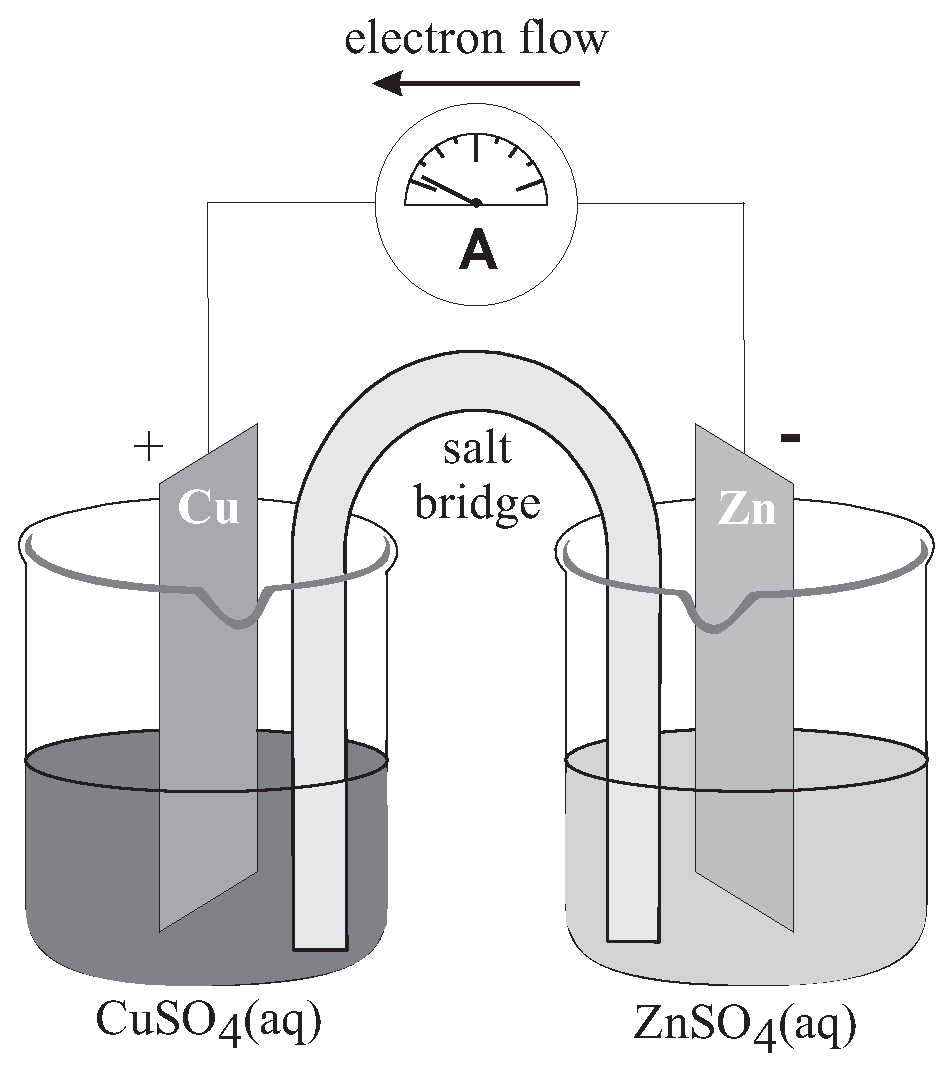
\includegraphics[width=6cm]{../../epsimages/VoltaicCellbw.eps}
\end{center}
}

\Results{

During the experiment, you should have noticed the following:

\begin{itemize}
\item{When the U-tube containing the Na$_{2}$SO$_{4}$ solution was absent, there was no reading on the ammeter.}
\item{When the U-tube was connected, a reading was recorded on the ammeter.}
\item{After the plates had been connected directly to each other and left for a day, there was a change in their mass. The mass of the zinc plate decreased, while the mass of the copper plate increased.}
\item{The direction of electron flow is from the zinc plate towards the copper plate.}
\end{itemize}
}

\Conclusions{

When a zinc sulphate solution containing a zinc plate is connected by a U-tube to a copper sulphate solution containing a copper plate, reactions occur in both solutions. The decrease in mass of the zinc plate suggests that the zinc metal has been oxidised. The increase in mass of the copper plate suggests that reduction has occurred here to produce more copper metal. This will be explained in detail below.}
}

\subsection{Half-cell reactions in the Zn-Cu cell}

The experiment above demonstrated a zinc-copper cell. This was made up of a zinc \textbf{half cell} and a copper \textbf{half cell}.

\Definition{Half cell}{
A half cell is a structure that consists of a conductive electrode surrounded by a conductive electrolyte. For example, a zinc half cell could consist of a zinc metal plate (the electrode) in a zinc sulphate solution (the electrolyte).
}

How do we explain what has just been observed in the zinc-copper cell?

\begin{itemize}
\item{\textit{Copper plate}

At the copper plate, there was an \textit{increase} in mass. This means that Cu$^{2+}$ ions from the copper sulphate solution were deposited onto the plate as atoms of copper metal. The half-reaction that takes place at the copper plate is:
\begin{center}
\rm${Cu^{2+} + 2e^{-} \rightarrow Cu}$ \textbf{(Reduction half reaction)}
\end{center}

Another shortened way to represent this copper half-cell is Cu$^{2+}$/Cu.
}

\item{\textit{Zinc plate}

At the zinc plate, there was a \textit{decrease} in mass. This means that some of the zinc goes into solution as Z$^{2+}$ ions. The electrons remain on the zinc plate, giving it a negative charge. The half-reaction that takes place at the zinc plate is:
\begin{center}
\rm${Zn \rightarrow Zn^{2+} + 2e^{-}}$ \textbf{(Oxidation half reaction)}
\end{center}

The shortened way to represent the zinc half-cell is Zn/Zn$^{2+}$.\\

The overall reaction is:

\begin{center}
\rm${Zn + Cu^{2+} + 2e^{-} \rightarrow Zn^{2+} + Cu + 2e^{-}}$ or, if we cancel the electrons:

\rm${Zn + Cu^{2+} \rightarrow Zn^{2+} + Cu}$ 
\end{center}

For this electrochemical cell, the standard notation is:
\begin{equation*}
Zn|Zn^{2+}||Cu^{2+}|Cu
\end{equation*}
where
\begin{eqnarray*}
  | &=& \rm{a \ phase \ boundary \ (solid/aqueous)}\\
  || & = & \rm{the \ salt \ bridge}
\end{eqnarray*}
}  
\end{itemize}

In the notation used above, the oxidation half-reaction at the anode is written on the left, and the reduction half-reaction at the cathode is written on the right. In the Zn-Cu electrochemical cell, the direction of current flow in the external circuit is from the zinc electrode (where there has been a build up of electrons) to the copper electrode.
 
\subsection{Components of the Zn-Cu cell}

In the zinc-copper cell, the copper and zinc plates are called the \textbf{electrodes}. The electrode where oxidation occurs is called the \textbf{anode}, and the electrode where reduction takes place is called the \textbf{cathode}. In the zinc-copper cell, the zinc plate is the anode and the copper plate is the cathode.

\Definition{Electrode}{An electrode is an electrical conductor that is used to make contact with a metallic part of a circuit. The anode is the electrode where oxidation takes place. The cathode is the electrode where reduction takes place. }

The zinc sulphate and copper sulphate solutions are called the \textbf{electrolyte} solutions.

\Definition{Electrolyte}{An electrolyte is a substance that contains free ions and which therefore behaves as an electrical conductor.}

The U-tube also plays a very important role in the cell. In the Zn/Zn$^{2+}$ half-cell, there is a build up of positive charge because of the release of electrons through oxidation. In the Cu$^{2+}$/Cu half-cell, there is a decrease in the positive charge because electrons are gained through reduction. This causes a movement of SO$_{4}^{2-}$ ions into the beaker where there are too many positive ions, in order to neutralise the solution. Without this, the flow of electrons in the outer circuit stops completely. The U-tube is called the \textbf{salt bridge}. The salt bridge acts as a transfer medium that allows ions to flow through without allowing the different solutions to mix and react. 

\Definition{Salt bridge}{A salt bridge, in electrochemistry, is a laboratory device that is used to connect the oxidation and reduction half-cells of a galvanic cell.}

\subsection{The Galvanic cell}

In the zinc-copper cell the important thing to notice is that the chemical reactions that take place at the two electrodes cause an electric current to flow through the outer circuit. In this type of cell, \textbf{chemical energy is converted to electrical energy}. These are called \textbf{galvanic cells}. The zinc-copper cell is one example of a galvanic cell. A galvanic cell (which is also sometimes referred to as a \textbf{voltaic} or \textbf{electrochemical} cell) consists of two metals that are connected by a salt bridge between the individual half-cells. A galvanic cell generates electricity using the reactions that take place at these two metals, each of which has a different \textbf{reaction potential}.\\

So what is meant by the 'reaction potential' of a substance? Every metal has a different half reaction and different dissolving rates. When two metals with different reaction potentials are used in a galvanic cell, a potential difference is set up between the two electrodes, and the result is a flow of current through the wire that connects the electrodes. In the zinc-copper cell, zinc has a higher reaction potential than copper and therefore dissolves more readily into solution. The metal 'dissolves' when it loses electrons to form positive metal ions. These electrons are then transferred through the connecting wire in the outer circuit. 

\Definition{Galvanic cell}{A galvanic (voltaic) cell is an electrochemical cell that uses a chemical reaction between two dissimilar electrodes dipped in an electrolyte, to generate an electric current.}

\begin{IFact}{It was the Italian physician and anatomist Luigi Galvani who marked the birth of electrochemistry by making a link between chemical reactions and electricity. In 1780, Galvani discovered that when two different metals (copper and zinc for example) were connected together and then both touched to different parts of a nerve of a frog leg at the same time, they made the leg contract. He called this "animal electricity". While many scientists accepted his ideas, another scientist, Alessandro Volta, did not. In 1800, because of his professional disagreement over the galvanic response that had been suggested by Luigi Galvani, Volta developed the \textit{voltaic pile}, which was very similar to the galvanic cell. It was the work of these two men that paved the way for all electrical batteries.}
\end{IFact}

\begin{wex}{Understanding galvanic cells\\}{
For the following cell:
\begin{center}
\begin{equation*}
Zn|Zn^{2+}||Ag^{+}|Ag
\end{equation*}
\end{center}
\begin{enumerate}
\item{Give the anode and cathode half-reactions.}
\item{Write the overall equation for the chemical reaction.}
\item{Give the direction of the current in the external circuit.}
\end{enumerate}
}

{\westep{Identify the oxidation and reduction reactions}

In the standard notation format, the oxidation reaction is written on the left and the reduction reaction on the right. So, in this cell, zinc is oxidised and silver ions are reduced.\\
\westep{Write the two half reactions}

Oxidation half-reaction:

\rm${Zn \rightarrow Zn^{2+} + 2e^{-}}$\\

Reduction half-reaction:

\rm${Ag^{+} + e^{-} \rightarrow Ag}$\\
\westep{Combine the half-reactions to get the overall equation.}

When you combine the two half-reactions, all the reactants must go on the left side of the equation and the products must go on the right side of the equation. The overall equation therefore becomes:

\begin{center}
$\rm{Zn + Ag^{+} + e^{-} \rightarrow Zn^{2+} + 2e^{-} + Ag}$
\end{center}

Note that this equation is not balanced. This will be discussed later in the chapter.\\
\westep{Determine the direction of current flow}

A build up of electrons occurs where oxidation takes place. This is at the zinc electrode. Current will therefore flow from the zinc electrode to the silver electrode.
}
\end{wex}

\subsection{Uses and applications of the galvanic cell}

The principles of the galvanic cell are used to make \textbf{electrical batteries}. In science and technology, a battery is a device that stores chemical energy and makes it available in an electrical form. Batteries are made of electrochemical devices such as one or more galvanic cells, fuel cells or flow cells. Batteries have many uses including in torches, electrical appliances (long-life alkaline batteries), digital cameras (lithium batteries), hearing aids (silver-oxide batteries), digital watches (mercury batteries) and military applications (thermal batteries). Refer to chapter \ref{chap:chemindustry} for more information on batteries.\\

The galvanic cell can also be used for \textbf{electroplating}. Electroplating occurs when an electrically conductive object is coated with a layer of metal using electrical current. Sometimes, electroplating is used to give a metal particular properties such as corrosion protection or wear resistance. At other times, it can be for aesthetic reasons for example in the production of jewellery. This will be discussed in more detail later in this chapter. 

\Exercise{Galvanic cells\\}{
\begin{enumerate}

\item{The following half-reactions take place in an electrochemical cell:

$\rm{Fe \rightarrow Fe^{3+} + 3e^{-}}$

$\rm{Fe^{2+} + 2e^{-} \rightarrow Fe}$\\

	\begin{enumerate}
	\item{Which is the oxidation half-reaction?}
	\item{Which is the reduction half-reaction?}
	\item{Name one oxidising agent.}
	\item{Name one reducing agent.}
	\item{Use standard notation to represent this electrochemical cell.}
	\end{enumerate}

}

\item{For the following cell:}

\begin{equation*}
Mg|Mg^{2+}||Mn^{2+}|Mn
\end{equation*}

	\begin{enumerate}
	
	\item{Give the cathode half-reaction.}
	\item{Give the anode half-reaction.}
	\item{Give the overall equation for the electrochemical cell.}
	\item{What metals could be used for the electrodes in this electrochemical cell?}
	\item{Suggest two electrolytes for this electrochemical cell.}
	\item{In which direction will the current flow?}
	\item{Draw a simple sketch of the complete cell.}
	\end{enumerate}

\item{For the following cell:}

\begin{equation*}
Sn|Sn^{2+}||Ag^{+}|Ag
\end{equation*}

\begin{enumerate}
	\item{Give the cathode half-reaction.}
	\item{Give the anode half-reaction.}
	\item{Give the overall equation for the electrochemical cell.}
	\item{Draw a simple sketch of the complete cell.}
	\end{enumerate}

\end{enumerate}

% Automatically inserted shortcodes - number to insert 3
\par \practiceinfo
\par \begin{tabular}[h]{cccccc}
% Question 1
(1.)	01qj	&
% Question 2
(2.)	01qk	&
% Question 3
(3.)	01qm	&
\end{tabular}
% Automatically inserted shortcodes - number inserted 3
}



% CHILD SECTION END 



% CHILD SECTION START 

\section{The Electrolytic cell}
\label{sec:electrochemical:electrolytic}

In section \ref{sec:electrochemical:galvanic}, we saw that a chemical reaction that involves a transfer of electrons, can be used to produce an electric current. In this section, we are going to see whether the 'reverse' process applies. In other words, is it possible to use an electric current to force a particular chemical reaction to occur, which would otherwise not take place? The answer is 'yes', and the type of cell that is used to do this, is called an \textbf{electrolytic cell}.

\Definition{Electrolytic cell}{An electrolytic cell is a type of cell that uses electricity to drive a non-spontaneous reaction.}

An electrolytic cell is activated by applying an electrical potential across the anode and cathode to force an internal chemical reaction between the ions that are in the electrolyte solution. This process is called \textbf{electrolysis}.

\Definition{Electrolysis}{In chemistry and manufacturing, electrolysis is a method of separating bonded elements and compounds by passing an electric current through them.}

\Activity{Demonstration}{The movement of coloured ions\\}{

A piece of filter paper is soaked in an ammonia-ammonium chloride solution and placed on a microscope slide. The filter paper is then connected to a supply of electric current using crocodile clips and connecting wire as shown in the diagram below. A line of copper chromate solution is placed in the centre of the filter paper. The colour of this solution is initially green-brown. \\

\begin{center}
\begin{pspicture}(-6,-2.3)(6,3.7)
%\psgrid
\psset{unit=0.8}
\rput(-7,0){
\pnode(0,0){A}
\pnode(5,0){B}
\pnode(5,0.5){C}
\pnode(0,0.5){D}
\pnode(1,3){E}
\pnode(6,3){F}
\pnode(6,2.5){G}
\psframe(A)(C)
\psline(D)(E)(F)(C)
\psline(B)(G)(F)
\psline(C)(D)
\psframe[fillstyle=solid,fillcolor=lightgray](2,0)(3,0.5)
\pspolygon[fillstyle=solid,fillcolor=lightgray](2,0.5)(3,3)(4,3)(3,0.5)
\psline[arrowsize=10pt,arrowinset=0,arrowlength=2.5]{->}(-0.5,-1)(-0.5,1.5)(1,1.5)
\psline[arrowsize=10pt,arrowinset=0,arrowlength=2.5]{<-}(5,1.5)(6.5,1.5)(6.5,-1)
\battery(-0.5,-1)(6.5,-1){}
\uput[u](3.5,3){copper chromate (green brown)}
\psline(3.5,3.2)(3.5,2.5)
\uput[d](3,-1.5){start of reaction}
\uput[u](0,1.5){\Large{\textbf{+}}}
\uput[u](6,1.5){\Large{\textbf{-}}}
\uput[ul](3,-0.8){\Large{\textbf{+}}}
\uput[ur](3,-0.8){\Large{\textbf{-}}}
}

\rput(1,0){
\pnode(0,0){A}
\pnode(5,0){B}
\pnode(5,0.5){C}
\pnode(0,0.5){D}
\pnode(1,3){E}
\pnode(6,3){F}
\pnode(6,2.5){G}
\psframe(A)(C)
\psline(D)(E)(F)(C)
\psline(B)(G)(F)
\psline(C)(D)
\psframe[fillstyle=solid,fillcolor=gray](3,0)(3.5,0.5)
\psframe[fillstyle=solid,fillcolor=lightgray](2,0)(3,0.5)
\psframe(1.5,0)(2,0.5)
\pspolygon[fillstyle=solid,fillcolor=lightgray](2,0.5)(3,3)(4,3)(3,0.5)
\pspolygon(1.5,0.5)(2.5,3)(3,3)(2,0.5)
\pspolygon[fillstyle=solid,fillcolor=gray](3,0.5)(3.5,0.5)(4.5,3)(4,3)

\psline[arrowsize=10pt,arrowinset=0,arrowlength=2.5]{->}(-0.5,-1)(-0.5,1.5)(1,1.5)
\psline[arrowsize=10pt,arrowinset=0,arrowlength=2.5]{<-}(5,1.5)(6.5,1.5)(6.5,-1)
\battery(-0.5,-1)(6.5,-1){}
\pcline{<-}(1,3.2)(2.5,3.2)
\aput{:U}{negative ions}
\pcline{->}(4.5,3.2)(6,3.2)
\aput{:U}{positive ions}
\uput[d](3,-1.5){after 20 minutes}
\uput[u](0,1.5){\Large{\textbf{+}}}
\uput[u](6,1.5){\Large{\textbf{-}}}
\uput[ul](3,-0.8){\Large{\textbf{+}}}
\uput[ur](3,-0.8){\Large{\textbf{-}}}
}
\end{pspicture}
\end{center}


The current is then switched on and allowed to run for about 20 minutes. After this time, the central coloured band disappears and is replaced by two bands, one yellow and the other blue, which seem to have separated out from the first band of copper chromate. \\

\textbf{Explanation:} 

\begin{itemize}
\item{The cell that is used to supply an electric current sets up a potential difference across the circuit, so that one of the electrodes is positive and the other is negative.}
\item{The chromate (CrO$_{4}^{2-}$) ions in the copper chromate solution are attracted to the positive electrode, while the Cu$^{2+}$ ions are attracted to the negative electrode.}
\end{itemize}

\textbf{Conclusion:\\}

The movement of ions occurs because the electric current in the outer circuit sets up a potential difference between the two electrodes.
}

Similar principles apply in the electrolytic cell, where substances that are made of ions can be broken down into simpler substances through electrolysis.

\subsection{The electrolysis of copper sulphate}

There are a number of examples of electrolysis. The electrolysis of copper sulphate is just one.

\Activity{Demonstration}{The electrolysis of copper sulphate\\}{

Two copper electrodes are placed in a solution of blue copper sulphate and are connected to a source of electrical current as shown in the diagram below. The current is turned on and the reaction is left for a period of time.\\

\begin{center}
\begin{pspicture}(-2,-0.2)(5,6.6)
%\psgrid
\rput(0,0){\psset{unit=2}\filledbeaker}
\psframe(0.25,1)(0.75,4.5)
\rput(2,0){\psframe(0.25,1)(0.75,4.5)}
\psline(0.5,4.5)(0.5,6)
\battery(0.5,6)(2.5,6){}
\psline(2.5,4.5)(2.5,6)
\uput[ul](0.5,4.5){\textbf{+}}
\uput[ur](2.5,4.5){\textbf{--}}
\uput[ul](1.4,6){\textbf{+}}
\uput[ur](1.6,6){\textbf{--}}
\uput[l](0,3){positive anode}
\psline(-0.1,3)(0.5,3)

\uput[r](3,3){negative cathode}
\psline(3.1,3)(2.5,3)

\uput[l](0,2){copper electrode}
\psline(-0.1,2)(0.5,2.2)
\uput[r](3,2){copper electrode}
\psline(3.1,2)(2.5,2.2)

\uput[r](3,0){CuSO$_4$ solution}
\psline(3.1,0.1)(1.5,0.1)

\rput(0.5,0.5){SO$_4^{2-}$}
\rput(2.5,0.5){Cu$^{2+}$}
\psarc{->}(1,1){0.4}{-90}{90}
\psarc{<-}(2,1){0.4}{90}{-90}

\end{pspicture}
\end{center}

\textbf{Observations:}

\begin{itemize}
\item{The initial blue colour of the solution remains unchanged.}
\item{It appears that copper has been \textit{deposited} on one of the electrodes but \textit{dissolved} from the other.\\}
\end{itemize}

\textbf{Explanation:\\}

\begin{itemize}
\item{At the negative cathode, positively charged Cu$^{2+}$ ions are attracted to the negatively charged electrode. These ions gain electrons and are reduced to form copper metal, which is deposited on the electrode. The half-reaction that takes place is as follows:

\begin{center}
\rm${Cu^{2+}(aq) + 2e^{-} \rightarrow Cu(s)}$ \textbf{(reduction half reaction)}
\end{center}
}

\item{At the positive anode, copper metal is oxidised to form Cu$^{2+}$ ions. This is why it appears that some of the copper has dissolved from the electrode. The half-reaction that takes place is as follows:

\begin{center}
\rm${Cu(s) \rightarrow Cu^{2+}(aq) + 2e^{-}}$ \textbf{(oxidation half reaction)}
\end{center}
}

\item{The amount of copper that is \textit{deposited} at one electrode is approximately the same as the amount of copper that is \textit{dissolved} from the other. The number of Cu$^{2+}$ ions in the solution therefore remains almost the same and the blue colour of the solution is unchanged.}
\end{itemize}

\textbf{Conclusion:}\\

In this demonstration, an electric current was used to split CuSO$_{4}$ into its component ions, Cu$^{2+}$ and SO$_{4}^{2-}$. This process is called \textit{electrolysis}.

}

\subsection{The electrolysis of water}

Water can also undergo electrolysis to form hydrogen gas and oxygen gas according to the following reaction:

\begin{center}
\rm${2H_{2}O(l) \rightarrow 2H_{2}(g) + O_{2}(g)}$
\end{center}

This reaction is very important because hydrogen gas has the potential to be used as an energy source. The electrolytic cell for this reaction consists of two electrodes (normally platinum metal), submerged in an electrolyte and connected to a source of electric current.\\

The reduction half-reaction that takes place at the cathode is as follows:
\begin{center}
\rm${2H_{2}O(l) + 2e^{-} \rightarrow H_{2}(g) + 2OH^{-}(aq)}$
\end{center}

The oxidation half-reaction that takes place at the anode is as follows:
\begin{center}
\rm${2H_{2}O(l) \rightarrow O_{2}(g) + 4H^{+}(aq) + 4e^{-}}$
\end{center}

\subsection{A comparison of galvanic and electrolytic cells}

It should be much clearer now that there are a number of differences between a \textit{galvanic} and an \textit{electrolytic} cell. Some of these differences have been summarised in table \ref{tab:electrochemical:comparison}.

\begin{table}[h]
\begin{center}
\begin{tabular}{|p{4cm}|p{4cm}|p{4cm}|}\hline
\textbf{Item} & \textbf{Galvanic cell} & \textbf{Electrolytic cell}\\\hline
Metals used for electrode & Two metals with different reaction potentials are used as electrodes & The same metal can be used for both the cathode and the anode \\\hline
Charge of the anode & negative & positive \\\hline
Charge of the cathode & positive & negative \\\hline
The electrolyte solution/s & The electrolyte solutions are kept separate from one another, and are connected only by a salt bridge & The cathode and anode are in the same electrolyte \\\hline
Energy changes & Chemical potential energy from chemical reactions is converted to electrical energy & An external supply of electrical energy causes a chemical reaction to occur \\\hline
Applications & Run batteries, electroplating & Electrolysis e.g. of water, NaCl \\\hline

\end{tabular}
\end{center}
\caption{A comparison of galvanic and electrolytic cells}
\label{tab:electrochemical:comparison}
\end{table} 

\Exercise{Electrolyis\\}{

\begin{enumerate}
\item{An electrolytic cell consists of two electrodes in a silver chloride (AgCl) solution, connected to a source of current. A current is passed through the solution and Ag$^{+}$ ions are reduced to a silver metal deposit on one of the electrodes.}
	\begin{enumerate}
	\item{Give the equation for the reduction half-reaction.}
	\item{Give the equation for the oxidation half-reacion.}
	\end{enumerate}

\item{Electrolysis takes place in a solution of molten lead bromide (PbBr) to produce lead atoms.}
	\begin{enumerate}
	\item{Draw a simple diagram of the electrolytic cell.}
	\item{Give equations for the half-reactions that take place at the anode and cathode, and include these in the diagram.}
	\item{On your diagram, show the direction in which current flows.}
	\end{enumerate}
\end{enumerate}

% Automatically inserted shortcodes - number to insert 2
\par \practiceinfo
\par \begin{tabular}[h]{cccccc}
% Question 1
(1.)	01qn	&
% Question 2
(2.)	01qp	&
\end{tabular}
% Automatically inserted shortcodes - number inserted 2
}



% CHILD SECTION END 



% CHILD SECTION START 

\section{Standard Electrode Potentials}
\label{sec:electrochemical:potentials}



If a voltmeter is connected in the circuit of an electrochemical cell, a reading is obtained. In other words, there is a \textbf{potential difference} between the two half cells. In this section, we are going to look at this in more detail to try to understand more about the \textbf{electrode potentials} of each of the electrodes in the cell. We are going to break this section down so that you build up your understanding gradually. Make sure that you understand each subsection fully before moving on, otherwise it might get confusing!

\subsection{The different reactivities of metals}
\label{subsec:electrochemical:metal reactivity}

All metals have different reactivities. When metals react, they give away electrons and form positive ions. But some metals do this more easily than others. Look at the following two half reactions:

\begin{center}
\rm${Zn \rightarrow Zn^{2+} + 2e^{-}}$

\rm${Cu \rightarrow Cu^{2+} + 2e^{-}}$
\end{center}

Of these two metals, zinc is more reactive and is more likely to give away electrons to form Zn$^{2+}$ ions in solution, than is copper.

\subsection{Equilibrium reactions in half cells}
\label{subsec:electrochemical:equilibrium reactions}

Let's think back to the Zn-Cu electrochemical cell. This cell is made up of two half cells and the reactions that take place at each of the electrodes are as follows:

\begin{center}
\rm${Zn \rightarrow Zn^{2+} + 2e^{-}}$

\rm${Cu^{2+} + 2e^{-} \rightarrow Cu}$
\end{center}

At the zinc electrode, the zinc metal loses electrons and forms Zn$^{2+}$ ions. The electrons are concentrated on the zinc metal while the Zn$^{2+}$ ions are in solution. But some of the ions will be attracted back to the negatively charged metal, will gain their electrons again and will form zinc metal. A \textbf{dynamic equilibrium} is set up between the zinc metal and the Zn$^{2+}$ ions in solution when the rate at which ions are \textit{leaving} the metal is equal to the rate at which they are \textit{joining} it again. The situation looks something like the diagram in figure \ref{fig:electrochemical:zinc}.

\begin{figure}[h]
\begin{center}
\begin{pspicture}(-2,1)(6,6)
%\psgrid[gridcolor=lightgray]
\psline(0,1)(0,4)
\psline(4,1)(4,4)
\psline(0,1)(4,1)
\psframe(1.5,2)(2.5,5)
\psline(0,3)(1.5,3)
\psline(2.5,3)(4,3)
\rput(1.8,3.5){\Large\textbf{-}}
\rput(1.9,4){\Large\textbf{-}}
\rput(2.1,3.7){\Large\textbf{-}}
\rput(1.7,3.2){\Large\textbf{-}}
\rput(2.3,4.4){\Large\textbf{-}}
\rput(2.3,4.3){\Large\textbf{-}}
\rput(1.9,2.2){\Large\textbf{-}}
\rput(1.7,3.2){\Large\textbf{-}}
\rput(2,3.4){\Large\textbf{-}}
\rput(2.4,2.4){\Large\textbf{-}}
\rput(2.3,2.3){\Large\textbf{-}}
\rput(2,2.5){\Large\textbf{-}}

\rput(2.9,2.3){\textbf{2+}}
\rput(2.8,1.5){\textbf{2+}}
\rput(2.3,1.8){\textbf{2+}}
\rput(1.6,1.5){\textbf{2+}}
\rput(1.3,2.6){\textbf{2+}}
\psline(3.2,2.3)(4.2,2.3)
\rput(6.2,2.3){Zn$^{2+}$ ions in solution}
\psline(2,4.5)(4.2,4.5)
\rput(5.3,4.5){zinc metal}
\psline(2,3.5)(4.2,3.5)
\rput(8,3.5){concentration of electrons on metal surface}
\end{pspicture}
\caption{Zinc loses electrons to form positive ions in solution. The electrons accumulate on the metal surface.}
\label{fig:electrochemical:zinc}
\end{center}
\end{figure}

The equilibrium reaction is represented like this:

\begin{center}
\rm${Zn^{2+}(aq) + 2e^{-} \rightleftharpoons Zn(s)}$
\end{center}

(NOTE: By convention, the ions are written on the \textit{left} hand side of the equation)\\

In the zinc half cell, the equilibrium lies far to the left because the zinc loses electrons easily to form Zn$^{2+}$ ions. We can also say that the zinc is \textit{oxidised} and that it is a strong \textit{reducing agent}.\\

At the copper electrode, a similar process takes place. The difference though is that copper is not as reactive as zinc and so it does not form ions as easily. This means that the build up of electrons on the copper electrode is less (figure \ref{fig:electrochemical:copper}). \\ 

\begin{figure}[h]
\begin{center}
\begin{pspicture}(-2,1)(6,6)
%\psgrid[gridcolor=lightgray]
\psline(0,1)(0,4)
\psline(4,1)(4,4)
\psline(0,1)(4,1)
\psframe(1.5,2)(2.5,5)
\psline(0,3)(1.5,3)
\psline(2.5,3)(4,3)
\rput(1.9,4){\Large\textbf{-}}
\rput(2.1,3.7){\Large\textbf{-}}
\rput(1.7,3.2){\Large\textbf{-}}
\rput(2.3,4.3){\Large\textbf{-}}
\rput(1.7,3.2){\Large\textbf{-}}
\rput(2.3,2.3){\Large\textbf{-}}
\rput(2,2.5){\Large\textbf{-}}

\rput(2.3,1.8){\textbf{2+}}
\rput(1.6,1.5){\textbf{2+}}
\psline(2.7,1.8)(4.2,1.8)
\rput(6.2,2.3){Cu$^{2+}$ ions in solution}
\psline(2,4.5)(4.2,4.5)
\rput(5.3,4.5){copper metal}
\psline(2,3.5)(4.2,3.5)
\rput(8,3.5){concentration of electrons on metal surface}
\end{pspicture}
\caption{Zinc loses electrons to form positive ions in solution. The electrons accumulate on the metal surface.}
\label{fig:electrochemical:copper}
\end{center}
\end{figure}

The equilibrium reaction is shown like this:

\begin{center}
\rm${Cu^{2+}(aq) + 2e^{-} \rightleftharpoons Cu(s)}$
\end{center}

The equation lies far to the right because most of the copper is present as copper metal rather than as Cu$^{2+}$ ions. In this half reaction, the Cu$^{2+}$ ions are \textit{reduced}.

\subsection{Measuring electrode potential}
\label{subsec:electrochemical:measuring electrode potential}

If we put the two half cells together, a potential difference is set up in two places in the Zn-Cu cell:
\begin{enumerate}
\item{There is a potential difference between the metal and the solution surrounding it because one is more negative than the other.}
\item{There is a potential difference between the Zn and Cu electrodes because one is more negative than the other.}
\end{enumerate}

It is the \textbf{potential difference} (recorded as a voltage) between the two electrodes that causes electrons, and therefore current, to flow from the more negative electrode to the less negative electrode.\\

The problem though is that we cannot measure the potential difference (voltage) between a metal and its surrounding solution in the cell. To do this, we would need to connect a voltmeter to both the metal and the solution, which is not possible. This means we cannot measure the exact \textbf{electrode potential} (E$^{o}$V) of a particular metal. The electrode potential describes the ability of a metal to give up electrons. And if the exact electrode potential of each of the electrodes involved can't be measured, then it is difficult to calculate the potential difference between them. But what we \textit{can} do is to try to describe the electrode potential of a metal \textit{relative} to another substance. We need to use a \textbf{standard reference electrode} for this.

\subsection{The standard hydrogen electrode}
\label{subsec:electrochemical:hydrogen electrode}

Before we look at the standard hydrogen electrode, it may be useful to have some more understanding of the ideas behind a 'reference electrode'. Refer to the Tip box on 'Understanding the ideas behind a reference electrode' before you read further.

\Tip{Understanding the ideas behind a reference electrode}{\textit{Adapted from www.chemguide.co.uk}\\

Let's say that you have a device that you can use to measure heights from some distance away. You want to use this to find out how tall a particular person is. Unfortunately, you can't see their feet because they are standing in long grass. Although you can't measure their absolute height, what you can do is to measure their height relative to the post next to them. Let's say that person A for example is 15 cm \textit{shorter} than the height of the post. You could repeat this for a number of other people (B and C). Person B is 30 cm shorter than the post and person C is 10 cm \textit{taller} than the post.

\begin{center}
\begin{pspicture}(-3,-5)(6,3)
%\psgrid[gridcolor=lightgray]
\def\stickman{
\pscircle(2,2){0.4}
\psline(2,1.6)(2,0.6)
\psline(2,0.6)(1.3,0)
\psline(2,0.6)(2.7,0)
\psline(1.5,1.2)(2.5,1.2)
}
\rput(0,0){\stickman}
\psline(0,0)(3.2,0)
\psframe[fillstyle=solid,fillcolor=darkgray](3.2,0)(3.5,2.7)
\rput(0,-0.3){\textbf{A}}
\rput(-2,-4){
\rput(0,0){\psset{unit=0.8}\stickman}
\psline(0,0)(3.2,0)
\psframe[fillstyle=solid,fillcolor=darkgray](3.2,0)(3.5,2.7)
\rput(0,-0.3){\textbf{B}}
}
\rput(2,-4){
\rput(0,0){\psset{unit=1.2}\stickman}
\psline(0,0)(3.2,0)
\psframe[fillstyle=solid,fillcolor=darkgray](3.2,0)(3.5,2.7)
\rput(0,-0.3){\textbf{C}}
}
\end{pspicture}
\end{center}

You could summarise your findings as follows:

\begin{center}
\begin{tabular}{|c|c|}\hline
\textbf{Person} & \textbf{Height relative to post (cm)}\\\hline
A & -15 \\\hline
B & -30 \\\hline
C & +10 \\\hline
\end{tabular}
\end{center}



Although you don't know any of their absolute heights, you can rank them in order, and do some very simple sums to work out exactly how much taller one is than another. For example, person C is 25 cm taller than A and 40 cm taller than B.
}

As mentioned earlier, it is difficult to measure the \textit{absolute} electrode potential of a particular substance, but we can use a reference electrode (similar to the 'post' in the Tip box example) that we use to calculate \textit{relative} electrode potentials for these substances. The reference elctrode that is used is the \textbf{standard hydrogen electrode} (figure \ref{fig:electrochemical:hydrogen electrode}).

\Definition{Standard hydrogen electrode\\}{
The standard hydrogen electrode is a redox electrode which forms the basis of the scale of oxidation-reduction potentials. The actual electrode potential of the hydrogen electrode is estimated to be 4.44 � $\pm$ 0.02 V at 25$^{0}$C, but its standard electrode potential is said to be zero at all temperatures so that it can be used as for comparison with other electrodes. The hydrogen electrode is based on the following redox half cell:

\begin{center}
   $\rm{2H^{+}(aq) + 2e^{-} \rightarrow H_{2}(g)}$
\end{center}
} % end of the definition

\begin{figure}[h]
\begin{center}
\scalebox{1.3} % Change this value to rescale the drawing.
{
\begin{pspicture}(0,-3.5848436)(10.2864065,3.5648437)
\psline[linewidth=0.04cm](4.4370313,1.6848439)(4.4379997,-2.5351562)
\psline[linewidth=0.04cm](7.657031,-2.5151563)(7.657031,1.6848439)
\psline[linewidth=0.04cm](4.597031,1.2048438)(7.48,1.2048438)
\psline[linewidth=0.04cm](7.48,1.2048438)(7.657031,1.3648437)
\psline[linewidth=0.04cm](4.597031,1.2048439)(4.44,1.3648437)
\psline[linewidth=0.04cm](5.74,-1.1151563)(6.4570312,-1.1151563)
\psline[linewidth=0.04cm](6.4570312,-1.1151563)(6.4370313,-0.0351562)
\psline[linewidth=0.04cm](5.977031,-0.31515622)(5.977031,-0.7551562)
\psline[linewidth=0.04cm](5.977031,-0.7551562)(6.217031,-0.7551562)
\psline[linewidth=0.04cm](6.217031,-0.7551562)(6.217031,-0.3351562)
\psline[linewidth=0.04cm](6.217031,-0.3351562)(5.977031,-0.3351562)
\psline[linewidth=0.04cm](6.077031,-0.3351562)(6.077031,3.5248437)
\psline[linewidth=0.04cm](6.4370313,-0.05515619)(6.257031,0.2448438)
\psline[linewidth=0.04cm](5.9370313,0.22484376)(5.9370313,3.0048437)
\psline[linewidth=0.04cm](6.2570314,0.22484376)(6.2370315,3.1648438)
\psline[linewidth=0.04cm](6.2370315,3.1448438)(5.7370315,3.5448437)
\psline[linewidth=0.04cm](5.9379997,3.0048437)(5.52,3.2848437)
\psline[linewidth=0.04cm](5.517031,3.2848437)(4.117031,3.2848437)
\psline[linewidth=0.04cm](5.7570314,3.5448437)(4.157031,3.5448437)
\psline[linewidth=0.04cm](4.32,2.8048437)(5.12,2.8048437)
\psline[linewidth=0.04cm](4.317031,2.5048437)(4.977031,2.5048437)
\psline[linewidth=0.04cm](4.96,2.5248437)(5.08,2.3248436)
\psline[linewidth=0.04cm](5.12,2.8048437)(5.317031,2.5048437)
\psline[linewidth=0.04cm](5.3170314,2.5048437)(5.32,-1.2551563)
\psline[linewidth=0.04cm](5.077031,2.324844)(5.08,-1.2751563)
\psline[linewidth=0.04cm](4.4379997,1.6848438)(4.22,1.9048438)
\psline[linewidth=0.04cm,arrowsize=0.05291667cm 2.0,arrowlength=1.4,arrowinset=0.4]{->}(3.8570313,2.6448438)(4.68,2.6448438)
\psline[linewidth=0.04cm,arrowsize=0.05291667cm 2.0,arrowlength=1.4,arrowinset=0.4]{<-cc}(3.96,3.4248438)(4.597031,3.4248438)
\psdots[dotsize=0.12](6.077031,3.3448436)
\psdots[dotsize=0.08,fillstyle=solid,dotstyle=o](5.9170313,-0.9551562)
\psdots[dotsize=0.08,fillstyle=solid,dotstyle=o](6.317031,-0.8151562)
\psdots[dotsize=0.08,fillstyle=solid,dotstyle=o](6.297031,-0.2751562)
\psdots[dotsize=0.08,fillstyle=solid,dotstyle=o](5.9570312,-0.0751562)
\psdots[dotsize=0.08,fillstyle=solid,dotstyle=o](6.057031,-0.9551562)
\usefont{T1}{ptm}{m}{n}
\rput(8.621407,0.4698438){\small [H$_3$O$^+$]}
\usefont{T1}{ptm}{m}{n}
\rput(8.676406,0.0098438){\small (1 mol.dm$^{-3}$)}
\usefont{T1}{ptm}{m}{n}
\rput(8.644531,-0.4501562){\small 25 $^{\circ}$C}
\psline[linewidth=0.04cm](4.4570312,-2.5151563)(7.657031,-2.5151563)
\usefont{T1}{ptm}{m}{n}
\rput(3.5492187,-0.5301562){\small Pt}
\usefont{T1}{ptm}{m}{n}
\rput(2.722656,2.6698437){\small H$_2$ gas}
\usefont{T1}{ptm}{m}{n}
\rput(2.2823439,2.1898437){\small (1 x atmosphereric pressure)}
\psline[linewidth=0.04cm](3.8170311,-0.49515623)(6.097031,-0.5351562)
\usefont{T1}{ptm}{m}{n}
\psline[linewidth=0.04cm](5.7370315,-1.1151563)(5.7170315,-0.04515625)
\psline[linewidth=0.04cm](5.722467,-0.045392893)(5.9315953,0.23508051)
\psarc[linewidth=0.04](5.63,-1.2451563){0.31}{180.0}{356.9872}
\psarc[linewidth=0.04](5.62,-1.2351563){0.54}{180.0}{356.9872}
\psline[linewidth=0.04cm](5.92,-1.2751563)(6.18,-1.2751563)
\psline[linewidth=0.04cm](7.658,1.6848438)(7.858,1.9048438)
\psline[linewidth=0.04cm](7.92,0.5048438)(6.82,0.5048438)
\end{pspicture} 
}
\end{center}
\caption{The standard hydrogen electrode}
\label{fig:electrochemical:hydrogen electrode}
\end{figure}

A standard hydrogen electrode consists of a platinum electrode in a solution containing H$^{+}$ ions. The solution (e.g. H$_{2}$SO$_{4}$) that contains the H$^{+}$ ions has a concentration of 1 mol.dm$^{-3}$. As the hydrogen gas bubbles over the platinum electrode, an equilibrium is set up between hydrogen molecules and hydrogen ions in solution. The reaction is as follows:

\begin{center}
\rm${2H^{+}(aq) + 2e^{-} \rightleftharpoons H_{2}(g)}$
\end{center}

The position of this equilibrium can change if you change some of the conditions (e.g. concentration, temperature). It is therefore important that the conditions for the standard hydrogen electrode are standardised as follows: pressure = 100 kPa (1atm); temperature = 298 K (25$^{0}$C) and concentration = 1 mol.dm$^{-3}$.

In order to \textit{use} the hydrogen electrode, it needs to be attached to the electrode system that you are investigating. For example, if you are trying to determine the electrode potential of copper, you will need to connect the copper half cell to the hydrogen electrode; if you are trying to determine the electrode potential of zinc, you will need to connect the zinc half cell to the hydrogen electrode and so on. Let's look at the examples of zinc and copper in more detail.

\begin{enumerate}
\item{\textbf{Zinc}

Zinc has a greater tendency than hydrogen to form ions, so if the standard hydrogen electrode is connected to the zinc half cell, the zinc will be relatively more negative because the electrons that are released when zinc is oxidised will accumulate on the metal. The equilibria on the two electrodes are as follows:

\begin{center}
\rm${Zn^{2+}(aq) + 2e^{-} \rightleftharpoons Zn(s)}$

\rm${2H^{+}(aq) + 2e^{-} \rightleftharpoons H_{2}(g)}$
\end{center}

In the zinc half-reaction, the equilibrium lies far to the left and in the hydrogen half-reaction, the equilibrium lies far to the right. A simplified representation of the cell is shown in figure \ref{fig:zinc hydrogen}. 

\begin{figure}[h]
\begin{center}
\begin{pspicture}(-2,0)(6,5)
%\psgrid[gridcolor=lightgray]
\psframe(0,0)(1,2)
\psframe(3,0)(4,2)
\psline(0.5,2)(0.5,4)

\psline(3.5,2)(3.5,4)
\psline(0.5,4)(1.5,4)
\psline(3.5,4)(2.5,4)
\pscircle(2,4){0.5}
\rput(2,4){\textbf{V}}
\rput(0.7,1.7){\Large\textbf{-}}
\rput(0.2,1.2){\Large\textbf{-}}
\rput(0.5, 0.5){\Large\textbf{-}}
\rput(3.7,1.7){\Large\textbf{-}}
\rput(3.2,1.2){\Large\textbf{-}}
\rput(3.5, 0.5){\Large\textbf{-}}
\rput(3.7,0.7){\Large\textbf{-}}
\rput(3.6,0.3){\Large\textbf{-}}
\rput(3.6,1.6){\Large\textbf{-}}
\rput(3.5,1){\Large\textbf{-}}
\rput(-1,1.5){H electrode}
\rput(-1,1.2){(less negative)}
\rput(6.5,1.5){Zn electrode with electrons}

\end{pspicture}
\end{center}
\caption{When zinc is connected to the standard hydrogen electrode, relatively few electrons build up on the platinum (hydrogen) electrode. There are lots of electrons on the zinc electrode.}
\label{fig:zinc hydrogen}
\end{figure}


The voltmeter measures the potential difference between the charge on these electrodes. In this case, the voltmeter would read 0.76 and would show that Zn is the negative electrode (i.e. it has a relatively higher number of electrons).
}

\item{\textbf{Copper}

Copper has a lower tendency than hydrogen to form ions, so if the standard hydrogen electrode is connected to the copper half cell, the hydrogen will be relatively more negative. The equilibria on the two electrodes are as follows:

\begin{center}
\rm${Cu^{2+}(aq) + 2e^{-} \rightleftharpoons Cu(s)}$

\rm${2H^{+}(aq) + 2e^{-} \rightleftharpoons H_{2}(g)}$
\end{center}

In the copper half-reaction, the equilibrium lies far to the right and in the hydrogen half-reaction, the equilibrium lies far to the left. A simplified representation of the cell is shown in figure \ref{fig:copper hydrogen}. 

\begin{figure}[h]
\begin{center}
\begin{pspicture}(-2,0)(6,5)
%\psgrid[gridcolor=lightgray]
\psframe(0,0)(1,2)
\psframe(3,0)(4,2)
\psline(0.5,2)(0.5,4)
\psline(3.5,2)(3.5,4)
\psline(0.5,4)(1.5,4)
\psline(3.5,4)(2.5,4)
\pscircle(2,4){0.5}
\rput(2,4){\textbf{V}}
\rput(0.7,1.7){\Large\textbf{-}}
\rput(0.2,1.2){\Large\textbf{-}}
\rput(0.5, 0.5){\Large\textbf{-}}
\rput(3.7,1.7){\Large\textbf{-}}
\rput(3.2,1.2){\Large\textbf{-}}
\rput(3.5, 0.5){\Large\textbf{-}}
\rput(0.7,0.7){\Large\textbf{-}}
\rput(0.6,0.3){\Large\textbf{-}}
\rput(0.6,1.6){\Large\textbf{-}}
\rput(0.5,1){\Large\textbf{-}}
\rput(-1,1.5){H electrode}
\rput(5,1.5){Cu electrode}
\end{pspicture}
\end{center}
\caption{When copper is connected to the standard hydrogen electrode, relatively few electrons build up on the copper electrode. There are lots of electrons on the hydrogen electrode.}
\label{fig:copper hydrogen}
\end{figure}


The voltmeter measures the potential difference between the charge on these electrodes. In this case, the voltmeter would read 0.34 and would show that Cu is the positive electrode (i.e. it has a relatively lower number of electrons).
} 
\end{enumerate}

% All good up to here - MH 26/04 - except for incorrect Tip usage but won't stop compile

\subsection{Standard electrode potentials}
\label{subsec:electrochemical:standard potentials}

The voltages recorded earlier when zinc and copper were connected to a standard hydrogen electrode are in fact the \textbf{standard electrode potentials} for these two metals. It is important to remember that these are not \textit{absolute} values, but are potentials that have been measured \textit{relative} to the potential of hydrogen if the standard hydrogen electrode is taken to be zero. 

\Tip{Conventions and voltage sign\\}{By convention, the hydrogen electrode is written on the \textit{left hand side} of the cell. The sign of the voltage tells you the sign of the metal electrode.\\

In the examples we used earlier, zinc's electrode potential is actually -0.76 and copper is +0.34. So, if a metal has a \textit{negative} standard electrode potential, it means it forms ions easily. The more negative the value, the easier it is for that metal to form ions. If a metal has a \textit{positive} standard electrode potential, it means it does not form ions easily. This will be explained in more detail below.} 

Luckily for us, we do not have to calculate the standard electrode potential for every metal. This has been done already and the results are recorded in a table of standard electrode potentials (table \ref{tab:electrochemical:table sep}).\\

\begin{table}
\begin{center}
\begin{tabular}{|l|l|}\hline 
\textbf{Half-Reaction}
&
\textbf{$E^{0}V$} \\ \hline\hline
$Li^{+} + e^{-} \rightleftharpoons Li$ & -3.04 \\ \hline
$K^{+} + e^{-} \rightleftharpoons K $& -2.92 \\ \hline
$Ba^{2+} + 2e^{-} \rightleftharpoons Ba $& -2.90 \\ \hline
$Ca^{2+} + 2e^{-} \rightleftharpoons Ca $& -2.87 \\ \hline
$Na^{+} + e^{-} \rightleftharpoons Na $& -2.71 \\ \hline
$Mg^{2+} + 2e^{-} \rightleftharpoons Mg $& -2.37 \\ \hline
$Mn^{2+} + 2e^{-} \rightleftharpoons Mn $& -1.18 \\ \hline
$2H2O + 2e^{-} \rightleftharpoons H_{2} (g) + 2 OH^{-} $& -0.83 \\ \hline
$Zn^{2+} + 2e^{-} \rightleftharpoons Zn $& -0.76 \\ \hline
$Cr^{2+} + 2e^{-} \rightleftharpoons Cr $& -0.74 \\ \hline
$Fe^{2+} + 2e^{-} \rightleftharpoons Fe $& -0.44 \\ \hline
$Cr^{3+} + 3e^{-} \rightleftharpoons Cr $& -0.41 \\ \hline
$Cd^{2+} + 2e^{-} \rightleftharpoons Cd $& -0.40\\ \hline
$Co^{2+} + 2e^{-} \rightleftharpoons Co $& -0.28 \\ \hline
$Ni^{2+} + 2e^{-} \rightleftharpoons Ni $& -0.25 \\ \hline
$Sn^{2+} + 2e^{-} \rightleftharpoons Sn $& -0.14 \\ \hline
$Pb^{2+} + 2e^{-} \rightleftharpoons Pb $& -0.13 \\ \hline
$Fe^{3+} + 3e^{-} \rightleftharpoons Fe $& -0.04 \\ \hline
$2H^{+} + 2e^{-} \rightleftharpoons H_{2} (g) $& \textbf{0.00} \\ \hline
$S + 2H^{+} + 2e^{-} \rightleftharpoons H_{2}S (g) $& 0.14 \\ \hline
$Sn^{4+} + 2e^{-} \rightleftharpoons Sn^{2+} $& 0.15 \\ \hline
$Cu^{2+} + e^{-} \rightleftharpoons Cu^{+} $& 0.16 \\ \hline
$SO_{4}^{2+} + 4H^{+} + 2e^{-} \rightleftharpoons SO_{2} (g) + 2H_{2}O $& 0.17 \\ \hline
$Cu^{2+} + 2e^{-} \rightleftharpoons Cu $& 0.34 \\ \hline
$2H_{2}O + O_{2} + 4e^{-} \rightleftharpoons 4OH^{-} $& 0.40 \\ \hline
$Cu^{+} + e^{-} \rightleftharpoons Cu $& 0.52 \\ \hline
$I_{2} + 2e^{-} \rightleftharpoons 2I^{-} $& 0.54 \\ \hline
$O_{2} (g) + 2H^{+} + 2e^{-} \rightleftharpoons H_{2}O_{2} $& 0.68 \\ \hline
$Fe^{3+} + e^{-} \rightleftharpoons Fe^{2+}  $& 0.77 \\ \hline
$NO_{3}^{-} + 2H^{+} + e^{-} \rightleftharpoons NO_{2} (g) + H_{2}O $& 0.78 \\ \hline
$Hg^{2+} + 2e^{-} \rightleftharpoons Hg (l) $& 0.78 \\ \hline
$Ag^{+} + e^{-} \rightleftharpoons Ag $& 0.80 \\ \hline
$NO_{3}^{-} + 4H^{+} +3 e^{-} \rightleftharpoons NO (g) + 2H_{2}O $& 0.96 \\ \hline
$Br_{2} + 2e^{-} \rightleftharpoons 2Br^{-} $& 1.06 \\ \hline
$O_{2} (g) + 4H^{+} + 4e^{-} \rightleftharpoons 2H_{2}O $& 1.23 \\ \hline
$MnO_{2} + 4H^{+} + 2e^{-} \rightleftharpoons Mn^{2+} + 2H_{2}O $& 1.28 \\ \hline
$Cr_{2}O_{7}^{2-} + 14H^{+} + 6e^{-} \rightleftharpoons 2Cr^{3+} + 7H_{2}O $& 1.33 \\ \hline
$Cl_{2} + 2e^{-} \rightleftharpoons 2Cl^{-} $& 1.36 \\ \hline
$Au^{3+} + 3e^{-} \rightleftharpoons Au $& 1.50 \\ \hline
$MnO_{4}^{-} + 8H^{+} + 5e^{-} \rightleftharpoons Mn^{2+} + 4H_{2}O $& 1.52 \\ \hline
$Co^{3+} + e^{-} \rightleftharpoons Co^{2+} $& 1.82 \\ \hline
$F_{2} + 2e^{-} \rightleftharpoons 2F^{-} $& 2.87 \\ \hline
\end{tabular}
\end{center}
\caption{Standard Electrode Potentials} 
\label{tab:electrochemical:table sep}
\end{table}

A few examples from the table are shown in table \ref{tab:electrochemical:table sep abbrev}. These will be used to explain some of the trends in the table of electrode potentials.

\begin{table}[h]
\begin{center}
\begin{tabular}{|l|l|}\hline 
\textbf{Half-Reaction}
&
\textbf{$E^{0}V$} \\ \hline\hline
$Li^{+} + e^{-} \rightleftharpoons Li$ & -3.04 \\ \hline
$Zn^{2+} + 2e^{-} \rightleftharpoons Zn $& -0.76 \\ \hline
$Fe^{3+} + 3e^{-} \rightleftharpoons Fe $& -0.04 \\ \hline
$2H^{+} + 2e^{-} \rightleftharpoons H_{2} (g) $& \textbf{0.00} \\ \hline
$Cu^{2+} + 2e^{-} \rightleftharpoons Cu $& 0.34 \\ \hline
$Hg^{2+} + 2e^{-} \rightleftharpoons Hg (l) $& 0.78 \\ \hline
$Ag^{+} + e^{-} \rightleftharpoons Ag $& 0.80 \\ \hline
\end{tabular}
\end{center}
\caption{A few examples from the table of standard electrode potentials}
\label{tab:electrochemical:table sep abbrev}
\end{table}

Refer to table \ref{tab:electrochemical:table sep abbrev} and notice the following trends:

\begin{itemize}
\item{Metals at the top of series (e.g. Li) have more negative values. This means they ionise easily, in other words, they release electrons easily. These metals are easily \textbf{oxidised} and are therefore good \textbf{reducing agents}.}
\item{Metal ions at the bottom of the table are good at picking up electrons. They are easily \textbf{reduced} and are therefore good \textbf{oxidising agents}.}
\item{The reducing ability (i.e. the ability to act as a reducing agent) of the metals in the table \textit{increases} as you move \textit{up} in the table.}
\item{The oxidising ability of metals \textit{increases} as you move \textit{down} in the table.}
\end{itemize}

\begin{wex}{Using the table of Standard Electrode Potentials\\}{

The following half-reactions take place in an electrochemical cell:

$\rm{Cu^{2+} + 2e^{-} \rightleftharpoons Cu}$

$\rm{Ag^{-} + e^{-} \rightleftharpoons Ag}$\\

	\begin{enumerate}
	\item{Which of these reactions will be the oxidation half-reaction in the cell?}
	\item{Which of these reactions will be the reduction half-reaction in the cell?}
	\end{enumerate}
}
{
\westep{Determine the electrode potential for each metal}

From the table of standard electrode potentials, the electrode potential for the copper half-reaction is +0.34 V. The electrode potential for the silver half-reaction is +0.80 V.\\

\westep{Use the electrode potential values to determine which metal is oxidised and which is reduced}

Both values are positive, but silver has a higher positive electrode potential than copper. This means that silver does not form ions easily, in other words, silver is more likely to be \textit{reduced}. Copper is more likely to be \textit{oxidised} and to form ions more easily than silver. Copper is the oxidation half-reaction and silver is the reduction half-reaction.
}
\end{wex}

\Tip{Learning to understand the question in a problem.\\ Before you tackle this problem, make sure you understand exactly what the question is asking. If magnesium is able to displace silver from a solution of silver nitrate, this means that magnesium metal will form magnesium ions and the silver ions will become silver metal. In other words, there will now be \textit{silver} metal and a solution of \textit{magnesium nitrate}. This will only happen if magnesium has a greater tendency than silver to form ions. In other words, what the question is actually asking is whether magnesium or silver forms ions more easily.
}

\begin{wex}{Using the table of Standard Electrode Potentials\\}{
Is magnesium able to displace silver from a solution of silver nitrate?}
{ % start answer

\westep{Determine the half-reactions that would take place if magnesium were to displace silver nitrate.}

The half-reactions are as follows:

\rm${Mg^{2+} + 2e^{-} \rightleftharpoons Mg}$

\rm${Ag^{+} + e^{-} \rightleftharpoons Ag}$\\

\westep{Use the table of electrode potentials to see which metal forms ions more easily.}

Looking at the electrode potentials for the magnesium and silver reactions: 

For the magnesium half-reaction: E$^{o}$V = -2.37

For the silver half-reaction: E$^{o}$V = 0.80\\

This means that magnesium is more easily \textbf{oxidised} than silver and the equilibrium in this half-reaction lies to the left. The oxidation reaction will occur spontaneously in magnesium. Silver is more easily \textbf{reduced} and the equilibrium lies to the right in this half-reaction. It can be concluded that magnesium will displace silver from a silver nitrate solution so that there is silver metal and magnesium ions in the solution.
}
\end{wex}

\Exercise{Table of Standard Electrode Potentials}
{
\begin{enumerate}
\item{In your own words, explain what is meant by the 'electrode potential' of a metal.}
\item{Give the standard electrode potential for each of the following metals:
	\begin{enumerate}
	\item{magnesium}
	\item{lead}
	\item{nickel}
	\end{enumerate}}
\item{Refer to the electrode potentials in table \ref{tab:electrochemical:table sep abbrev}.
	\begin{enumerate}
	\item{Which of the metals is most likely to be oxidised?}
	\item{Which metal is most likely to be reduced?}
	\item{Which metal is the strongest reducing agent?}
	\item{In the copper half-reaction, does the equilibrium position for the reaction lie to the left or to the right? Explain your answer.}
	\item{In the mercury half-reaction, does the equilibrium position for the reaction lie to the left or to the right? Explain your answer.}
	\item{If silver was added to a solution of copper sulphate, would it displace the copper from the copper sulphate solution? Explain your answer.}
	\end{enumerate}}
\item{Use the table of standard electrode potentials to put the following in order from the \textit{strongest oxidising agent} to the \textit{weakest oxidising agent}.
	\begin{itemize}
	\item{Cu$^{2+}$}
	\item{MnO$_{4}^{-}$}
	\item{Br$_{2}$}
	\item{Zn$^{2+}$}
	\end{itemize}}
\item{Look at the following half-reactions.
	\begin{itemize}
	\item{\rm${Ca^{2+} + 2e^{-} \rightarrow Ca}$}
	\item{\rm${Cl_{2} + 2e^{-} \rightarrow 2Cl}$}
	\item{\rm${Fe^{3+} + 3e^{-} \rightarrow Fe}$}
	\item{\rm${I_{2} + 2e^{-} \rightarrow 2I^{-}}$}
 	\end{itemize}

	\begin{enumerate}
	\item{Which substance is the strongest oxidising agent?}
	\item{Which substance is the strongest reducing agent?}
	\end{enumerate}}

\item{Which one of the substances listed below acts as the oxidising agent in the following reaction?
\begin{center}
$\rm{3SO_{2} + Cr_{2}O_{7}^{2-} + 2H^{+} \rightarrow 3SO_{4}^{2-} + 2Cr^{3+} + H_{2}O}$
\end{center}
	\begin{enumerate}
	\item{H$^{+}$}
	\item{Cr$^{3+}$}
	\item{SO$_{2}$}
	\item{Cr$_{2}$O$_{7}^{2-}$}
	\end{enumerate}
(IEB Paper 2, 2004)
}
\item{If zinc is added to a solution of magnesium sulphate, will the zinc displace the magnesium from the solution? Give a detailed explanation for your answer.}
\end{enumerate}

% Automatically inserted shortcodes - number to insert 7
\par \practiceinfo
\par \begin{tabular}[h]{cccccc}
% Question 1
(1.)	01qq	&
% Question 2
(2.)	01qr	&
% Question 3
(3.)	01qs	&
% Question 4
(4.)	01qt	&
% Question 5
(5.)	01qu	&
% Question 6
(6.)	01qv	\\ % End row of shortcodes
% Question 7
(7.)	01qw	&
\end{tabular}
% Automatically inserted shortcodes - number inserted 7


} % end of Exercise


\subsection{Combining half cells}
\label{subsec:electrochemical:combining half cells}

Let's stay with the example of the zinc and copper half cells. If we combine these cells as we did earlier in the chapter (section \ref{sec:electrochemical:galvanic}), the following two equilibria exist:

\begin{center}
\rm${Zn^{2+} + 2e^{-} \rightleftharpoons Zn (E^{0} = -0.76V)}$

\rm${Cu^{2+} + 2e^{-} \rightleftharpoons Cu (E^{0} = +0.34V)}$
\end{center}

We know from demonstrations, and also by looking at the sign of the electrode potential, that when these two half cells are combined, zinc will be the oxidation half-reaction and copper will be the reduction half-reaction. A voltmeter connected to this cell will show that the zinc electrode is more negative than the copper electrode. The reading on the meter will show the potential difference between the two half cells. This is known as the \textbf{electromotive force (emf)} of the cell.

\Definition{Electromotive Force (emf)}{The emf of a cell is defined as the maximum potential difference between two electrodes or half cells in a voltaic cell. emf is the electrical driving force of the cell reaction. In other words, the higher the emf, the stronger the reaction.}

\Definition{Standard emf (E$^{0}_{cell}$)}{Standard emf is the emf of a voltaic cell operating under standard conditions (i.e. 100 kPa, concentration = 1 mol.dm$^{-3}$ and temperature = 298 K). The symbol $^{0}$ denotes standard conditions.}

When we want to represent this cell, it is shown as follows:

\begin{center}
\begin{equation*}
Zn|Zn^{2+} (1 mol.dm^{-3})||Cu^{2+} (1 mol.dm^{-3})|Cu
\end{equation*}
\end{center}

The \textbf{anode} half cell (where \textit{oxidation} takes place) is always written on the \textit{left}. The \textbf{cathode} half cell (where \textit{reduction} takes place) is always written on the \textit{right}.

It is important to note that the potential difference across a cell is related to the extent to which the spontaneous cell reaction has reached equilibrium. In other words, as the reaction proceeds and the concentration of reactants decreases and the concentration of products increases, the reaction approaches equilibrium. When equilibrium is reached, the emf of the cell is zero and the cell is said to be 'flat'. There is no longer a potential difference between the two half cells, and therefore no more current will flow. 

\subsection{Uses of standard electrode potential}
\label{subsec:electrochemical:uses of sep}

Standard electrode potentials have a number of different uses.

%\begin{enumerate} % PROBLEM!!! - going to try to make the items subsubsections
%\item{\textbf{Calculating the emf of an electrochemical cell}

\subsubsection{Calculating the emf of an electrochemical cell}

To calculate the emf of a cell, you can use any one of the following equations:

E$^{0}_{(cell)}$ = E$^{0}$ (right) - E$^{0}$ (left) ('right' refers to the electrode that is written on the right in standard cell notation. 'Left' refers to the half-reaction written on the left in this notation) 

E$^{0}_{(cell)}$ = E$^{0}$ (reduction half reaction) - E$^{0}$ (oxidation half reaction)

E$^{0}_{(cell)}$ = E$^{0}$ (oxidising agent) - E$^{0}$ (reducing agent)

E$^{0}_{(cell)}$ = E$^{0}$ (cathode) - E$^{0}$ (anode)


So, for the Zn-Cu cell, \\

E$^{0}_{(cell)}$ = 0.34 - (-0.76)

= 0.34 + 0.76

= 1.1 V

%}

\begin{wex}{Calculating the emf of a cell}{The following reaction takes place:

\begin{center}
\rm${Cu(s) + Ag^{+}(aq) \rightarrow Cu^{2+}(aq) + Ag(s)}$
\end{center}

\begin{enumerate}
\item{Represent the cell using standard notation.}
\item{Calculate the cell potential (emf) of the electrochemical cell.\\}
\end{enumerate}
}
{
\westep{Write equations for the two half reactions involved}
\rm${Cu^{2+} + 2e^{-} \rightleftharpoons Cu}$ (E$^{o}$V = 0.16V)

\rm${Ag^{+} + e^{-} \rightleftharpoons Ag}$ (E$^{o}$V = 0.80V)\\

\westep{Determine which reaction takes place at the cathode and which is the anode reaction}
Both half-reactions have positive electrode potentials, but the silver half-reaction has a higher positive value. In other words, silver does not form ions easily, and this must be the reduction half-reaction. Copper is the oxidation half-reaction. Copper is oxidised, therefore this is the anode reaction. Silver is reduced and so this is the cathode reaction.

\westep{Represent the cell using standard notation}
\begin{equation*}
Cu|Cu^{2+} (1 mol.dm^{-3})||Ag^{+} (1 mol.dm^{-3})|Ag
\end{equation*}

\westep{Calculate the cell potential}
E$^{0}_{(cell)}$ = E$^{0}$ (cathode) - E$^{0}$ (anode)

= +0.80 - (+0.34)

= +0.46 V\\
}
\end{wex}

\begin{wex}{Calculating the emf of a cell}{Calculate the cell potential of the electrochemical cell in which the following reaction takes place, and represent the cell using standard notation.

\begin{center}
\rm${Mg(s) + 2H^{+}(aq) \rightarrow Mg{2+}(aq) + H_{2}(g)}$
\end{center}
}

{\westep{Write equations for the two half reactions involved}
\rm${Mg^{2+} + 2e^{-} \rightleftharpoons Mg}$ (E$^{o}$V = -2.37)

\rm${2H^{+} + 2e^{-} \rightleftharpoons H_{2}}$ (E$^{o}$V = 0.00)\\

\westep{Determine which reaction takes place at the cathode and which is the anode reaction}
From the overall equation, it is clear that magnesium is oxidised and hydrogen ions are reduced in this reaction. Magnesium is therefore the anode reaction and hydrogen is the cathode reaction.

\westep{Represent the cell using standard notation}
\begin{equation*}
Mg|Mg^{2+}||H^{+}|H_{2}
\end{equation*}

\westep{Calculate the cell potential}
E$^{0}_{(cell)}$ = E$^{0}$ (cathode) - E$^{0}$ (anode)

= 0.00 - (-2.37)

= +2.37 V
}
\end{wex}

%\item{\textbf{Predicting whether a reaction will take place spontaneously}\\
\subsubsection{Predicting whether a reaction will take place spontaneously}

Look at the following example to help you to understand how to predict whether a reaction will take place spontaneously or not.

In the reaction,

\begin{center}
\rm${Pb^{2+}(aq) + 2Br^{-}(aq) \rightarrow Br_{2}(l) + Pb(s)}$
\end{center}

the two half reactions are as follows:

\begin{center}
\rm${Pb^{2+} + 2e^{-} \rightleftharpoons Pb}$ (-0.13 V)

\rm${Br_{2} + 2e^{-} \rightleftharpoons 2Br^{-}}$ (+1.06 V)
\end{center}

\Tip{Half cell reactions}{You will see that the half reactions are written as they appear in the table of standard electrode potentials. It may be useful to highlight the reacting substance in each half reaction. In this case, the reactants are Pb$^{2+}$ and Br$^{-}$ ions.}

Look at the electrode potential for the first half reaction. The negative value shows that lead loses electrons easily, in other words it is easily oxidised. The reaction would normally proceed from right to left (i.e. the equilibrium lies to the left), but in the original equation, the opposite is happening. It is the Pb$^{2+}$ ions that are being reduced to lead. This part of the reaction is therefore not spontaneous. The positive electrode potential value for the bromine half-reaction shows that bromine is more easily reduced, in other words the equilibrium lies to the right. The spontaneous reaction proceeds from left to right. This is not what is happening in the original equation and therefore this is also not spontaneous. Overall it is clear then that the reaction will not proceed spontaneously.

\begin{wex}{Predicting whether a reaction is spontaneous}{Will copper react with dilute sulfuric acid (H$_{2}$SO$_{4}$)? You are given the following half reactions:

\begin{center}
\rm${Cu^{2+}(aq) + 2e^{-} \rightleftharpoons Cu(s)}$ (E$^{0}$ = +0.34 V)

\rm${2H^{+}(aq) + 2e^{-} \rightleftharpoons H_{2}(g)}$ (E$^{0}$ = 0 V)
\end{center} 
}
{\westep{For each reaction, look at the electrode potentials and decide in which direction the equilibrium lies}
In the first half reaction, the positive electrode potential means that copper does not lose electrons easily, in other words it is more easily reduced and the equilibrium position lies to the right. Another way of saying this is that the spontaneous reaction is the one that proceeds from left to right, when copper ions are reduced to copper metal.

In the second half reaction, the spontaneous reaction is from right to left.

\westep{Compare the equilibrium positions to the original reaction}

What you should notice is that in the original reaction, the reactants are copper (Cu) and sulfuric acid (2H$^{+}$). During the reaction, the copper is oxidised and the hydrogen ions are reduced. But from an earlier step, we know that neither of these half reactions will proceed spontaneously in the direction indicated by the original reaction. The reaction is therefore not spontaneous.
}
\end{wex} 

\Tip{}{\textbf{A second method for predicting whether a reaction is spontaneous}

Another way of predicting whether a reaction occurs spontaneously, is to look at the sign of the emf value for the cell. If the emf is \textbf{positive} then the reaction is \textbf{spontaneous}. If the emf is \textbf{negative}, then the reaction is \textbf{not spontaneous}.
} % end Tip

%\item{\textbf{Balancing redox reactions}
\subsubsection{Balancing redox reactions}

We will look at this in more detail in the next section.


%}
%\end{enumerate}

\Exercise{Predicting whether a reaction will take place spontaneously\\}{
\begin{enumerate}
\item Predict whether the following reaction will take place spontaneously or not. Show all your working.
\begin{equation*}
2Ag (s) + Cu^{2+} (aq) \rightarrow Cu (s) + 2Ag^{+} (aq)
\end{equation*}

\item Zinc metal reacts with an acid, H$^{+}$ (aq) to produce hydrogen gas.
	\begin{enumerate}
	\item{Write an equation for the reaction, using the table of electrode potentials.}
	\item{Predict whether the reaction will take place spontaneously. Show your working.}
	\end{enumerate}

\item Four beakers are set up, each of which contains one of the following solutions:
	\begin{enumerate}
	\item{Mg(NO$_{3}$)$_{2}$}
	\item{Ba(NO$_{3}$)$_{2}$}
	\item{Cu(NO$_{3}$)$_{2}$}
	\item{Al(NO$_{3}$)$_{2}$}
	\end{enumerate}

Iron is added to each of the beakers. In which beaker will a spontaneous reaction take place?

\item Which one of the following solutions can be stored in an aluminium container?
	\begin{enumerate}
	\item{Cu(SO)$_{4}$}
	\item{Zn(SO)$_{4}$}
	\item{NaCl}
	\item{Pb(NO$_{3}$)$_{2}$}
	\end{enumerate}
\end{enumerate}

% Automatically inserted shortcodes - number to insert 4
\par \practiceinfo
\par \begin{tabular}[h]{cccccc}
% Question 1
(1.)	01qx	&
% Question 2
(2.)	01qy	&
% Question 3
(3.)	01qz	&
% Question 4
(4.)	01r0	&
\end{tabular}
% Automatically inserted shortcodes - number inserted 4
} % End of exercise


\Exercise{Electrochemical cells and standard electrode potentials}{

\begin{enumerate}
\item An electrochemical cell is made up of a copper electrode in contact with a copper nitrate solution and an electrode made of an unknown metal M in contact with a solution of MNO$_{3}$. A salt bridge containing a KNO$_{3}$ solution joins the two half cells. A voltmeter is connected across the electrodes. Under standard conditions the reading on the voltmeter is 0.46V.

\begin{center}
\begin{pspicture}(-4,-3)(5,2)
\rput(-2,0){
%\psgrid[gridcolor=lightgray]
\psset{unit=0.7}
\psline[linewidth=3pt](-1,0.5)(-1,-3.5)
\psline[linewidth=3pt](-1,-3.5)(2,-3.5)
\psline[linewidth=3pt](2,-3.5)(2,0.5)
\psframe[fillstyle=solid,fillcolor=gray](0,-3)(0.5,2)
\psline[linewidth=0.6pt](0.25,2)(0.25,2.5)
\psline[linewidth=0.6pt](0.25,2.5)(4,2.5)
\psline[linewidth=0.6pt](4,2.5)(4,2)
\psellipse(2,2.5)(0.5,0.5)
\rput(2,2.5){\textbf{V}}
\psline(0,1.5)(-2,1.5)
\rput(-3,1.5){Cu}
\rput(3.75,0){
\psline[linewidth=3pt](-1,0.5)(-1,-3.5)
\psline[linewidth=3pt](-1,-3.5)(2,-3.5)
\psline[linewidth=3pt](2,-3.5)(2,0.5)
\psframe[fillstyle=solid,fillcolor=gray](0,-3)(0.5,2)

}
\psline(-1,-0.75)(0,-0.75)
\psline(0.5,-0.75)(2,-0.75)
\psline(2.75,-0.75)(3.75,-0.75)
\psline(4.25,-0.75)(5.75,-0.75)

\psline[linewidth=2pt](1.3,-1.5)(1.3,1)
\psline[linewidth=2pt](1.3,1)(3.3,1)
\psline[linewidth=2pt](3.3,1)(3.3,-1.5)

\rput(2.1,1.5){Salt bridge (KNO$_{3}$)}

\psline(0,-2)(-2,-2)
\rput(-3.4,-2){Cu(NO$_{3}$)$_{2}$ (aq)}
\psline(4.25,-2)(6,-2)
\rput(7.3,-2){MNO$_{3}$(aq)}
\psline(4.25,1.5)(6,1.5)
\rput(6.5,1.5){M}

}
\end{pspicture}
\end{center}

The reaction in the copper half cell is given by:

$\rm{Cu \rightarrow Cu^{2+} + 2e^{-}}$\\

	\begin{enumerate}
	\item{Write down the standard conditions which apply to this electrochemical cell.}
	\item{Identify the metal M. Show calculations.}
	\item Use the standard electrode potentials to write down equations for the:
		\begin{enumerate}
		\item{cathode half-reaction}
		\item{anode half-reaction}
		\item{overall cell reaction}
		\end{enumerate}
	\item{What is the purpose of the salt bridge?}
	\item{Explain why a KCl solution would not be suitable for use in the salt bridge in this cell.}
	\end{enumerate}

(IEB Paper 2, 2004)

\item Calculate the emf for each of the following standard electrochemical cells:

	\begin{enumerate}

\item 
\begin{equation*}
Mg|Mg^{2+}||H^{+}|H_{2}
\end{equation*}

\item
\begin{equation*}
Fe|Fe^{3+}||Fe^{2+}|Fe
\end{equation*}


\item
\begin{equation*}
Cr|Cr{2+}||Cu^{2+}|Cu
\end{equation*}


\item
\begin{equation*}
Pb|Pb^{2+}||Hg^{2+}|Hg
\end{equation*}

\end{enumerate}

\item Given the following two half-reactions:

	\begin{itemize}
	\item{\rm${Fe^{3+}(aq) + e^{-} \rightleftharpoons Fe^{2+}(aq)}$}
	\item{\rm${MnO_{4}^{-}(aq) + 8H^{+}(aq) + 5e^{-} \rightleftharpoons Mn^{2+}(aq) + 4H_{2}O(l)}$}
	\end{itemize}

	\begin{enumerate}
	\item{Give the standard electrode potential for each half-reaction.}
	\item{Which reaction takes place at the cathode and which reaction takes place at the anode?}
	\item{Represent the electrochemical cell using standard notation.}
	\item{Calculate the emf of the cell}
	\end{enumerate}

\end{enumerate}

% Automatically inserted shortcodes - number to insert 3
\par \practiceinfo
\par \begin{tabular}[h]{cccccc}
% Question 1
(1.)	01r1	&
% Question 2
(2.)	01r2	&
% Question 3
(3.)	01r3	&
\end{tabular}
% Automatically inserted shortcodes - number inserted 3

}


% CHILD SECTION END 



% CHILD SECTION START 

\section{Balancing redox reactions}
\label{sec:electrochemical:balancing}

Half reactions can be used to balance redox reactions. We are going to use some worked examples to help explain the method.

\begin{wex}{Balancing redox reactions\\}{Magnesium reduces copper (II) oxide to copper. In the process, magnesium is oxidised to magnesium ions. Write a balanced equation for this reaction.\\}

{\westep{Write down the unbalanced oxidation half reaction.}

\begin{center}
\rm${Mg \rightarrow Mg^{2+}}$\\
\end{center}
\westep{Balance the number of atoms on both sides of the equation.} 

You are allowed to add hydrogen ions (H$^{+}$) and water molecules if the reaction takes place in an acid medium. If the reaction takes place in a basic medium, you can add either hydroxide ions (OH$^{-}$) or water molecules. In this case, there is one magnesium atom on the left and one on the right, so no additional atoms need to be added.\\
\westep{Once the atoms are balanced, check that the \textit{charges} balance.}

Charges can be balanced by adding electrons to either side. The charge on the left of the equation is 0, but the charge on the right is +2. Therefore, two electrons must be added to the right hand side so that the charges balance. The half reaction is now:

\begin{center}
\rm${Mg \rightarrow Mg^{2+} + 2e^{-}}$\\
\end{center}
\westep{Repeat the above steps, but this time using the reduction half reaction.}

The reduction half reaction is:

\begin{center}
\rm${Cu^{2+} \rightarrow Cu}$
\end{center}

The atoms balance but the charges don't. Two electrons must be added to the right hand side.

\begin{center}
\rm${Cu^{2+} + 2e^{-} \rightarrow Cu}$\\
\end{center}
\westep{Multiply each half reaction by a suitable number so that the number of electrons \textit{released} in the oxidation half reaction is made equal to the number of electrons that are accepted in the reduction half reaction.}

No multiplication is needed because there are two electrons on either side.\\
\westep{Combine the two half reactions to get a final equation for the overall reaction.}

\begin{center}
\rm${Mg + Cu^{2+} + 2e^{-} \rightarrow Mg^{2+} + Cu + 2e^{-}}$ (The electrons on either side cancel and you get...)

\rm${Mg + Cu^{2+} \rightarrow Mg^{2+} + Cu}$\\
\end{center}
\westep{Do a final check to make sure that the equation is balanced}

In this case, it is.
}
\end{wex}


\begin{wex}{Balancing redox reactions\\}{Chlorine gas oxidises Fe(II) ions to Fe(III) ions. In the process, chlorine is reduced to chloride ions. Write a balanced equation for this reaction.\\}

{\westep{Write down the oxidation half reaction.}

\begin{center}
\rm${Fe^{2+} \rightarrow Fe^{3+}}$\\
\end{center}
\westep{Balance the number of atoms on both sides of the equation.} 

There is one iron atom on the left and one on the right, so no additional atoms need to be added.\\
\westep{Once the atoms are balanced, check that the \textit{charges} balance.}

The charge on the left of the equation is +2, but the charge on the right is +3. Therefore, one electron must be added to the right hand side so that the charges balance. The half reaction is now:

\begin{center}
\rm${Fe^{2+} \rightarrow Fe^{3+} + e^{-}}$\\
\end{center}
\westep{Repeat the above steps, but this time using the reduction half reaction.}

The reduction half reaction is:

\begin{center}
\rm${Cl_{2} \rightarrow Cl^{-}}$
\end{center}

The atoms don't balance, so we need to multiply the right hand side by two to fix this. Two electrons must be added to the left hand side to balance the charges.

\begin{center}
\rm${Cl_{2} + 2e^{-} \rightarrow 2Cl^{-}}$
\end{center}
\westep{Multiply each half reaction by a suitable number so that the number of electrons \textit{released} in the oxidation half reaction is made equal to the number of electrons that are accepted in the reduction half reaction.}

We need to multiply the oxidation half reaction by two so that the number of electrons on either side are balanced. This gives:

\begin{center}
\rm${2Fe^{2+} \rightarrow 2Fe^{3+} + 2e^{-}}$\\
\end{center}
\westep{Combine the two half reactions to get a final equation for the overall reaction.}

\begin{center}
\rm${2Fe^{2+} + Cl_{2} \rightarrow 2Fe^{3+} + 2Cl^{-}}$\\
\end{center}
\westep{Do a final check to make sure that the equation is balanced}
The equation is balanced.
}
\end{wex}

\begin{wex}{Balancing redox reactions in an acid medium\\}{The following reaction takes place in an acid medium:

\begin{center}
\rm${Cr_{2}O_{7}^{2-} + H_{2}S \rightarrow Cr^{3+} + S}$
\end{center}

Write a balanced equation for this reaction.\\}

{\westep{Write down the oxidation half reaction.}

\begin{center}
\rm${Cr_{2}O_{7}^{2-} \rightarrow Cr^{3+}}$\\
\end{center}
\westep{Balance the number of atoms on both sides of the equation.} 

We need to multiply the right side by two so that the number of Cr atoms will balance. To balance the oxygen atoms, we will need to add water molecules to the right hand side. 

\begin{center}
\rm${Cr_{2}O_{7}^{2-} \rightarrow 2Cr^{3+} + 7H_{2}O}$
\end{center}

Now the oxygen atoms balance but the hydrogens don't. Because the reaction takes place in an acid medium, we can add hydrogen ions to the left side.

\begin{center}
\rm${Cr_{2}O_{7}^{2-} + 14H^{+} \rightarrow 2Cr^{3+} + 7H_{2}O}$\\
\end{center}
\westep{Once the atoms are balanced, check that the \textit{charges} balance.}

The charge on the left of the equation is (-2+14) = +12, but the charge on the right is +6. Therefore, six electrons must be added to the left hand side so that the charges balance. The half reaction is now:

\begin{center}
\rm${Cr_{2}O_{7}^{2-} + 14H^{+} + 6e^{-} \rightarrow 2Cr^{3+} + 7H_{2}O}$\\
\end{center}
\westep{Repeat the above steps, but this time using the reduction half reaction.}

The reduction half reaction after the charges have been balanced is:

\begin{center}
\rm${S^{2-} \rightarrow S + 2e^{-}}$\\
\end{center}
\westep{Multiply each half reaction by a suitable number so that the number of electrons \textit{released} in the oxidation half reaction is made equal to the number of electrons that are accepted in the reduction half reaction.}

We need to multiply the reduction half reaction by three so that the number of electrons on either side are balanced. This gives:

\begin{center}
\rm${3S^{2-} \rightarrow 3S + 6e^{-}}$\\
\end{center}
\westep{Combine the two half reactions to get a final equation for the overall reaction.}

\begin{center}
\rm${Cr_{2}O_{7}^{2-} + 14H^{+} + 3S^{2-} \rightarrow 3S + 2Cr^{3+} + 7H_{2}O}$\\
\end{center}
\westep{Do a final check to make sure that the equation is balanced}
}
\end{wex}

\begin{wex}{Balancing redox reactions in an alkaline medium\\}{If ammonia solution is added to a solution that contains cobalt(II) ions, a complex ion is formed, called the hexaaminecobalt(II) ion (Co(NH$_{3}$)$_{6}^{2+}$). In a chemical reaction with hydrogen peroxide solution, hexaaminecobalt ions are oxidised by hydrogen peroxide solution to the hexaaminecobalt(III) ion Co(NH$_{3}$)$_{6}^{3+}$. Write a balanced equation for this reaction.\\}

{\westep{Write down the oxidation half reaction}

\begin{center}
\rm${Co(NH_{3})_{6}^{2+} \rightarrow Co(NH_{3})_{6}^{3+}}$\\
\end{center}
\westep{Balance the number of atoms on both sides of the equation.} 

The number of atoms are the same on both sides.\\
\westep{Once the atoms are balanced, check that the \textit{charges} balance.}

The charge on the left of the equation is +2, but the charge on the right is +3. One elctron must be added to the right hand side to balance the charges in the equation.The half reaction is now:

\begin{center}
\rm${Co(NH_{3})_{6}^{2+} \rightarrow Co(NH_{3})_{6}^{3+} + e^{-}}$\\
\end{center}
\westep{Repeat the above steps, but this time using the reduction half reaction.}

Although you don't actually know what product is formed when hydrogen peroxide is reduced, the most logical product is OH$^{-}$. The reduction half reaction is:

\begin{center}
\rm${H_{2}O_{2} \rightarrow OH^{-}}$\\
\end{center}

After the atoms and charges have been balanced, the final equation for the reduction half reaction is:

\begin{center}
\rm${H_{2}O_{2} + 2e^{-} \rightarrow 2OH^{-}}$\\
\end{center}
\westep{Multiply each half reaction by a suitable number so that the number of electrons \textit{released} in the oxidation half reaction is made equal to the number of electrons that are accepted in the reduction half reaction.}

We need to multiply the oxidation half reaction by two so that the number of electrons on both sides are balanced. This gives:

\begin{center}
\rm${2Co(NH_{3})_{6}^{2+} \rightarrow 2Co(NH_{3})_{6}^{3+} + 2e^{-}}$\\
\end{center}
\westep{Combine the two half reactions to get a final equation for the overall reaction.}

\begin{center}
\rm${2Co(NH_{3})_{6}^{2+} + H_{2}O_{2} \rightarrow 2Co(NH_{3})_{6}^{3+} + 2OH^{-}}$\\
\end{center}
\westep{Do a final check to make sure that the equation is balanced}
}
\end{wex}

\Exercise{Balancing redox reactions\\}{
\begin{enumerate}
\item{Balance the following equations.}
	\begin{enumerate}
	\item{\rm${HNO_{3} + PbS \rightarrow PbSO_{4} + NO + H_{2}O}$}
	\item{\rm${NaI + Fe_{2}(SO_{4})_{3} \rightarrow I_{2} + FeSO_{4} + Na_{2}SO_{4}}$}
		\end{enumerate}

\item{Manganate(VII) ions (MnO$_{4}^{-}$) oxidise hydrogen peroxide (H$_{2}$O$_{2}$) to oxygen gas. The reaction is done in an acid medium. During the reaction, the manganate(VII) ions are reduced to manganese(II) ions (Mn$^{2+}$). Write a balanced equation for the reaction.}

\item{Chlorine gas is prepared in the laboratory by adding concentrated hydrochloric acid to manganese dioxide powder. The mixture is carefully heated.}
	\begin{enumerate}
	\item{Write down a balanced equation for the reaction which takes place.}
	\item{Using standard electrode potentials, show by calculations why this mixture needs to be heated.}
	\item{Besides chlorine gas which is formed during the reaction, hydrogen chloride gas is given off when the conentrated hydrochloric acid is heated. Explain why the hydrogen chloride gas is removed from the gas mixture when the gas is bubbled through water.}

(IEB Paper 2, 2004) 
	\end{enumerate}

\item{The following equation can be deduced from the table of standard electrode potentials:}
\begin{center}
$\rm{2Cr_{2}O_{7}^{2-}(aq) + 16H^{+} (aq) \rightarrow 4Cr^{3+} (aq) + 3O_{2} (g) + 8H_{2}O (l)}$ (E$^{0}$ = +0.10V)
\end{center}

This equation implies that an acidified solution of aqueous potassium dichromate (orange) should react to form Cr$^{3+}$ (green). Yet aqueous laboratory solutions of potassium dichromate remain orange for years. Which ONE of the following best explains this?

	\begin{enumerate}
	\item{Laboratory solutions of aqueous potassium dichromate are not acidified}
	\item{The E$^{0}$ value for this reaction is only +0.10V}
	\item{The activation energy is too low}
	\item{The reaction is non-spontaneous}
	\end{enumerate}

(IEB Paper 2, 2002)

\item{Sulfur dioxide gas can be prepared in the laboratory by heating a mixture of copper turnings and concentrated sulfuric acid in a suitable flask.}	
	\begin{enumerate}
	\item{Derive a balanced ionic equation for this reaction using the half-reactions that take place.}
	\item{Give the E$^{0}$ value for the overall reaction.}
	\item{Explain why it is necessary to heat the reaction mixture.}
	\item{The sulfur dioxide gas is now bubbled through an aqueous solution of potassium dichromate. Describe and explain what changes occur during this process.}
	\end{enumerate}
(IEB Paper 2, 2002)
\end{enumerate}

% Automatically inserted shortcodes - number to insert 5
\par \practiceinfo
\par \begin{tabular}[h]{cccccc}
% Question 1
(1.)	01r4	&
% Question 2
(2.)	01r5	&
% Question 3
(3.)	01r6	&
% Question 4
(4.)	01r7	&
% Question 5
(5.)	01r8	&
\end{tabular}
% Automatically inserted shortcodes - number inserted 5

}


% CHILD SECTION END 



% CHILD SECTION START 

\section{Applications of electrochemistry}
\label{sec:electrochemical:applications}

Electrochemistry has a number of different uses, particularly in industry. We are going to look at a few examples.

\subsection{Electroplating}

Electroplating is the process of using electrical current to coat an electrically conductive object with a thin layer of metal. Mostly, this application is used to deposit a layer of metal that has some desired property (e.g. abrasion and wear resistance, corrosion protection, improvement of aesthetic qualities etc.) onto a surface that doesn't have that property. Electro-refining (also sometimes called \textit{electrowinning} is electroplating on a large scale. Electrochemical reactions are used to deposit pure metals from their ores. One example is the electrorefining of copper.\\

Copper plays a major role in the electrical reticulation industry as it is very conductive and is used in electric cables. One of the problems though is that copper must be pure if it is to be an effective current carrier. One of the methods used to purify copper, is electrowinning. The copper electrowinning process is as follows:

\begin{enumerate}
  \item Bars of crude (impure) copper containing other metallic
  impurities is placed on the \emph{anodes}.
  \item The \emph{cathodes} are made up of pure copper with few impurities.
  \item The electrolyte is a solution of aqueous $CuSO_{4}$ and $H_{2}SO_{4}$.
  \item When current passes through the cell, electrolysis takes place. The impure copper anode dissolves to form Cu$^{2+}$ ions in solution. These positive ions are attracted to the negative cathode, where reduction takes place to produce pure copper metal. The reactions that take place are as follows:

At the \emph{anode}:
\begin{equation*}
Cu(s) \rightarrow Cu^{2+}(aq) + 2e^{-}
  \end{equation*}

At the \emph{cathode}:
\begin{equation*}
Cu^{+2}(aq) + 2e^{-} \rightarrow Cu(s) \rm{ \ \ \ \ \ } (> 99\% purity)
\end{equation*}

  \item The other metal impurities (Zn, Au, Ag, Fe and Pb) do not
  dissolve and form a solid sludge at the bottom of the tank or
  remain in solution in the electrolyte.
\end{enumerate}

\begin{figure}[h]
\begin{center}
\begin{pspicture}(-2,-0.2)(5,6.6)
%\psgrid
\rput(0,0){\psset{unit=2}\filledbeaker}
\psframe(0.25,1)(0.75,4.5)
\rput(2,0){\psframe(0.25,1)(0.75,4.5)}
\psline(0.5,4.5)(0.5,6)
\battery(0.5,6)(2.5,6){}
\psline(2.5,4.5)(2.5,6)
\uput[ul](0.5,4.5){\textbf{+}}
\uput[ur](2.5,4.5){\textbf{--}}
\uput[ul](1.4,6){\textbf{+}}
\uput[ur](1.6,6){\textbf{--}}
\uput[l](0,3){positive anode}
\psline(-0.1,3)(0.5,3)

\uput[r](3,3){negative cathode}
\psline(3.1,3)(2.5,3)

\uput[l](0,2){impure copper electrode}
\psline(-0.1,2)(0.5,2.2)
\uput[r](3,2){pure copper electrode}
\psline(3.1,2)(2.5,2.2)

\rput(1.5,1.5){Cu$^{2+}$}
\psline[arrows=->](1,1)(2,1)
\end{pspicture}
\caption{A simplified diagram to illustrate what happens during the electrowinning of copper}
\label{fig:electrochemical:electrowinning}
\end{center}
\end{figure}



\subsection{The production of chlorine}

Electrolysis can also be used to produce chlorine gas from brine/seawater (NaCl). This is sometimes referred to as the 'Chlor-alkali' process. The reactions that take place are as follows:\\

At the \emph{anode} the reaction is:
\begin{eqnarray*}
2Cl^{-}  \rightarrow Cl_{2}(g) + 2e^{-} \\
\end{eqnarray*}

whereas at the \emph{cathode}, the following happens:
\begin{eqnarray*}
2Na^{+} + 2H_{2}O + 2e^{-}   \rightarrow 2Na^{+} + 2OH^{-} + H_{2} \\
\end{eqnarray*}

The overall reaction is:
\begin{eqnarray*}
2Na^{+} + 2H_{2}O + 2Cl^{-} \rightarrow 2Na^{+} + 2OH^{-} + H_{2} + Cl_{2} \\
\end{eqnarray*}

\begin{figure}[h]
\begin{center}
\begin{pspicture}(-2,-0.2)(5,6.6)
%\psgrid
\rput(0,0){\psset{unit=2}\filledbeaker}
\psframe(0.25,1)(0.75,4.5)
\rput(2,0){\psframe(0.25,1)(0.75,4.5)}
\psline(0.5,4.5)(0.5,6)
\battery(0.5,6)(2.5,6){}
\psline(2.5,4.5)(2.5,6)
\uput[ul](0.5,4.5){\textbf{+}}
\uput[ur](2.5,4.5){\textbf{--}}
\uput[ul](1.4,6){\textbf{+}}
\uput[ur](1.6,6){\textbf{--}}
\uput[l](0,3){positive anode}
\psline(-0.1,3)(0.5,3)

\uput[r](3,3){negative cathode}
\psline(3.1,3)(2.5,3)

\uput[l](0,2){electrode}
\psline(-0.1,2)(0.5,2.2)
\uput[r](3,2){electrode}
\psline(3.1,2)(2.5,2.2)

\uput[r](3,0){NaCl solution}
\psline(3.1,0.1)(1.5,0.1)

\rput(0.5,0.5){Cl$^{-}$}
\rput(2.5,0.5){Na$^{+}$}
\psarc{->}(1,1){0.4}{-90}{90}
\psarc{<-}(2,1){0.4}{90}{-90}

\end{pspicture}
\end{center}
\caption{The electrolysis of sodium chloride}
\label{fig:electrochemical:nacl}
\end{figure}

Chlorine is a very important chemical. It is used as a bleaching agent, a disinfectant, in solvents, pharmaceuticals, dyes and even plastics such as polyvinlychloride (PVC).

\subsection{Extraction of aluminium}

Aluminum metal is a commonly used metal in industry where its properties of being both light and strong can be utilized. It is also used in the manufacture of products such as aeroplanes and motor cars. The metal is present in
deposits of bauxite which is a mixture of silicas, iron oxides and hydrated alumina ($Al_{2}O_{3}$ x $H_{2}O$). \\

Electrolysis can be used to extract aluminum from bauxite. The process described below produces $99\%$ pure aluminum:

\begin{enumerate}


  \item Aluminum is melted along with cryolite ($Na_{3}AlF_{6}$) which acts as the electrolyte. Cryolite helps to lower the melting point and dissolve the ore.
  \item  The \emph{anode} carbon rods provide sites for the oxidation of $O^{2-}$
  and $F^{-}$ ions. Oxygen and flourine gas are given off at the anodes and
  also lead to anode consumption.
  \item At the \emph{cathode} cell lining, the $Al^{3+}$ ions are reduced and metal
  aluminum deposits on the lining.
  \item The $AlF_{6}^{3-}$ electrolyte is stable and remains in its molten state.
\end{enumerate}

The basic electrolytic reactions involved are as follows:
At the \emph{cathode}:
\begin{eqnarray*}
  Al^{+3} + 3e^{-} &\rightarrow& Al(s) \rm{ \ \ \ \ \ } (99\% purity)
  \end{eqnarray*}

At the \emph{anode}:
\begin{eqnarray*}
  2O^{2-} &\rightarrow& O_{2}(g) + 4e^{-}
\end{eqnarray*}

The overall reaction is as follows:
\begin{eqnarray*}
  2Al_{2}O_{3} &\rightarrow& 4Al + 3O_{2}
\end{eqnarray*}

The only problem with this process is that the reaction is \textit{endothermic} and large amounts of electricity are needed to drive the reaction. The process is therefore very expensive.

\summary{aaa}

\begin{itemize}
\item{An \textbf{electrochemical reaction} is one where either a chemical reaction produces an external voltage, or where an external voltage causes a chemical reaction to take place.}
\item{In a \textbf{galvanic cell} a chemical reaction produces a current in the external circuit. An example is the zinc-copper cell.}
\item{A galvanic cell has a number of \textbf{components}. It consists of two \textbf{electrodes}, each of which is placed in a separate beaker in an \textbf{electrolyte} solution. The two electrolytes are connected by a \textbf{salt bridge}. The electrodes are connected two each other by an external circuit wire.}
\item{One of the electrodes is the \textbf{anode}, where \textbf{oxidation} takes place. The \textbf{cathode} is the electrode where \textbf{reduction} takes place.}
\item{In a galvanic cell, the build up of electrons at the anode sets up a potential difference between the two electrodes, and this causes a \textbf{current} to flow in the external circuit.}   
\item{A \textbf{galvanic cell} is therefore an electrochemical cell that uses a chemical reaction between two dissimilar electrodes dipped in an electrolyte to generate an electric current.}
\item{The standard notation for a galvanic cell such as the zinc-copper cell is as follows:

\begin{equation*}
Zn|Zn^{2+}||Cu^{2+}|Cu
\end{equation*}
where
\begin{eqnarray*}
  | &=& \rm{a \ phase \ boundary \ (solid/aqueous)}\\
  || & = & \rm{the \ salt \ bridge}
\end{eqnarray*}
}
\item{The galvanic cell is used in \textbf{batteries} and in \textbf{electroplating}.}
\item{An \textbf{electrolytic cell} is an electrochemical cell that uses electricity to drive a non-spontaneous reaction. In an electrolytic cell, \textbf{electrolysis} occurs, which is a process of separating elements and compounds using an electric current.}
\item{One example of an electrolytic cell is the electrolysis of copper sulphate to produce copper and sulphate ions.}
\item{Different metals have different \textbf{reaction potentials}. The reaction potential of metals (in other words, their ability to ionise), is recorded in a \textbf{standard table of electrode potential}. The more negative the value, the greater the tendency of the metal to be oxidised. The more positive the value, the greater the tendency of the metal to be reduced.}
\item{The values on the standard table of electrode potentials are measured relative to the \textbf{standard hydrogen electrode}.}
\item{The emf of a cell can be calculated using one of the following equations:

E$^{0}_{(cell)}$ = E$^{0}$ (right) - E$^{0}$ (left)

E$^{0}_{(cell)}$ = E$^{0}$ (reduction half reaction) - E$^{0}$ (oxidation half reaction)

E$^{0}_{(cell)}$ = E$^{0}$ (oxidising agent) - E$^{0}$ (reducing agent)

E$^{0}_{(cell)}$ = E$^{0}$ (cathode) - E$^{0}$ (anode)
}
\item{It is possible to predict whether a reaction is \textbf{spontaneous} or not, either by looking at the sign of the cell's emf or by comparing the electrode potentials of the two half cells.}
\item{It is possible to \textbf{balance} redox equations using the half-reactions that take place.}
\item{There are a number of important \textbf{applications} of electrochemistry. These include \textbf{electroplating}, the \textbf{production of chlorine} and the \textbf{extraction of aluminium}.}
\end{itemize}

\begin{eocexercises}{}

\begin{enumerate}

\item{For each of the following, say whether the statement is \textbf{true} or \textbf{false}. If it is false, re-write the statement correctly.}
	\begin{enumerate}
	\item{The anode in an electrolytic cell has a negative charge.}
	\item{The reaction $\rm{2KClO_{3} \rightarrow 2KCl + 3O_{2}}$ is an example of a redox reaction.}
	\item{Lead is a stronger oxidising agent than nickel.}
	\end{enumerate}

\item{For each of the following questions, choose the \textbf{one correct} answer.}

	\begin{enumerate}
	\item{Which one of the following reactions is a redox reaction?}
		\begin{enumerate}
		\item{\rm${HCl + NaOH \rightarrow NaCl + H_{2}O}$}
		\item{\rm${AgNO_{3} + NaI \rightarrow AgI + NaNO_{3}}$}
		\item{\rm${2FeCl_{3} + 2H_{2}O + SO_{2} \rightarrow H_{2}SO_{4} + 2HCl + 2FeCl_{2}}$}
		\item{\rm${BaCl_{2} + MgSO_{4} \rightarrow MgCl_{2} + BaSO_{4}}$}
		\end{enumerate}
(IEB Paper 2, 2003) 
	\item{Consider the reaction represented by the following equation:\\

\rm${Br_{2(l)} + 2I^{-}_{aq} \rightarrow 2Br^{-}_{aq} + I_{2(s)}}$\\

Which one of the following statements about this reaction is correct?}
	
		\begin{enumerate}
		\item{bromine is oxidised}
		\item{bromine acts as a reducing agent}
		\item{the iodide ions are oxidised}
		\item{iodine acts as a reducing agent}
		\end{enumerate}

(IEB Paper 2, 2002)

	\item{The following equations represent two hypothetical half-reactions:\\

\rm${X_{2} + 2e^{-} \rightleftharpoons 2X^{-}}$ (+1.09 V) and

\rm${Y^{+} + e^{-} \rightleftharpoons Y}$ (-2.80 V)\\

Which one of the following substances from these half-reactions has the greatest tendency to donate electrons?}

		\begin{enumerate}
		\item{X$^{-}$}
		\item{X$_{2}$}
		\item{Y}
		\item{Y$^{+}$}
		\end{enumerate}


	\item{Which one of the following redox reactions will \textbf{not} occur spontaneously at room temperature?}

		\begin{enumerate}
		\item{\rm${Mn + Cu^{2+} \rightarrow Mn^{2+} + Cu}$}
		\item{\rm${Zn + SO_{4}^{2-} + 4H^{+} \rightarrow Zn^{2+} + SO_{2} + 2H_{2}O}$}
		\item{\rm${Fe^{3+} + 3NO_{2} + 3H_{2}O \rightarrow Fe + 3NO_{3}^{-} + 6H^{+}}$}
		\item{\rm${5H_{2}S + 2MnO_{4}^{-} + 6H^{+}\rightarrow 5S + 2Mn^{2+} + 8H_{2}O}$}
		\end{enumerate}

	\item{Which statement is CORRECT for a Zn-Cu galvanic cell that operates under standard conditions?}
		\begin{enumerate}
		\item{The concentration of the Zn$^{2+}$ ions in the zinc half-cell gradually decreases.}
		\item{The concentration of the Cu$^{2+}$ ions in the copper half-cell gradually increases.}
		\item{Negative ions migrate from the zinc half-cell to the copper half-cell.}
		\item{The intensity of the colour of the electrolyte in the copper half-cell gradually decreases.}
		\end{enumerate}
(DoE Exemplar Paper 2, 2008)

	\end{enumerate}


\item{In order to investigate the rate at which a reaction proceeds, a learner places a beaker containing concentrated nitric acid on a sensitive balance. A few pieces of copper metal are dropped into the nitric acid. }
	\begin{enumerate}
	\item{Use the relevant half-reactions from the table of Standard Reduction Potentials to derive the balanced nett ionic equation for the reaction that takes place in the beaker.}
	\item{What chemical property of nitric acid is illustrated by this reaction?}
	\item{List three observations that this learner would make during the investigation.}
	\end{enumerate}
(IEB Paper 2, 2005)
\item{The following reaction takes place in an electrochemical cell:
\begin{equation*}
Cu(s) + 2AgNO_{3}(aq) \rightarrow Cu(NO_{3})_{2}(aq) + 2Ag(s)
\end{equation*}

	\begin{enumerate}
	\item{Give an equation for the oxidation half reaction.}
	\item{Which metal is used as the anode?}
	\item{Determine the emf of the cell under standard conditions.}
	\end{enumerate}
}
(IEB Paper 2, 2003)
\item{The nickel-cadmium (NiCad) battery is small and light and is made in a sealed unit. It is used in portable appliances such as calculators and electric razors. The following two half reactions occur when electrical energy is produced by the cell.}

Half reaction 1: $\rm{Cd(s) + 2OH^{-}(aq) \rightarrow Cd(OH)_{2}(s) + 2e^{-}}$\\

Half reaction 2: $\rm{NiO(OH)(s) + H_{2}O(l) + e^{-} \rightarrow Ni(OH)_{2}(s) + OH^{-}(aq)}$

	\begin{enumerate}
	\item{Which half reaction (1 or 2) occurs at the anode? Give a reason for your answer.}
	\item{Which substance is oxidised?}
	\item{Derive a balanced ionic equation for the overall cell reaction for the discharging process.}
	\item{Use your result above to state in which direction the cell reaction will proceed (forward or reverse) when the cell is being charged.}
	\end{enumerate}

(IEB Paper 2, 2001)

\item{An electrochemical cell is constructed by placing a lead rod in a porous pot containing a solution of lead nitrate (see sketch). The porous pot is then placed in a large aluminium container filled with a solution of aluminium sulphate. The lead rod is then connected to the aluminium container by a copper wire and voltmeter as shown.}


\begin{center}
\begin{pspicture}(-4,-4)(3,2)
%\psgrid[gridcolor=lightgray]
\psset{unit=0.8}
\rput(-2,0){
\psline(-4,1)(-4,-4)
\psline(-4,-4)(4,-4)
\psline(4,-4)(4,1)
\psline(-4,0)(4,0)
\psline[linewidth=3pt](-1,0.5)(-1,-3.5)
\psline[linewidth=3pt](-1,-3.5)(2,-3.5)
\psline[linewidth=3pt](2,-3.5)(2,0.5)
\psframe[fillstyle=solid,fillcolor=gray](0,-3)(0.5,2)
\psline[linewidth=0.6pt](0.25,2)(0.25,2.5)
\psline[linewidth=0.6pt](0.25,2.5)(4,2.5)
\psline[linewidth=0.6pt](4,2.5)(4,1)
\psellipse(2,2.5)(0.5,0.5)
\rput(2,2.5){\small{\textbf{V}}}
\psline(4,1.5)(5,1.5)
\rput(6,1.5){\small{copper wire}}
\psline(4,-2)(5,-2)
\rput(6.7,-2){\small{aluminium container}}
\rput(1.25,-2){\small{Pb(NO$_{3}$)$_{2}$}}
\rput(1.2,-2.4){\small{(aq)}}
\rput(-2.5,-2){\small{Al$_{2}$(SO$_{4}$)$_{3}$ (aq)}}
\psline(-1,-1)(-2,-1)
\rput(-3,-1){\small{porous pot}}
\psline(0,1.5)(-2,1.5)
\rput(-3,1.5){\small{lead rod}}
}
\end{pspicture}
\end{center}

	\begin{enumerate}
	\item{Define the term \textit{reduction}.}
	\item{In which direction do electrons flow in the copper wire? (Al to Pb or Pb to Al)}
	\item{Write balanced equations for the reactions that take place at...}
		\begin{enumerate}
		\item{the anode}
		\item{the cathode}
		\end{enumerate}

	\item{Write a balanced nett ionic equation for the reaction which takes place in this cell.}
	\item{What are the two functions of the porous pot?}
	\item{Calculate the emf of this cell under standard conditions.}
	\end{enumerate}


(IEB Paper 2, 2005) 

\end{enumerate}
% Automatically inserted shortcodes - number to insert 6
\par \practiceinfo
\par \begin{tabular}[h]{cccccc}
% Question 1
(1.)	01r9	&
% Question 2
(2.)	01ra	&
% Question 3
(3.)	01rb	&
% Question 4
(4.)	01rc	&
% Question 5
(5.)	01rd	&
% Question 6
(6.)	01re	\\ % End row of shortcodes
\end{tabular}
% Automatically inserted shortcodes - number inserted 6
\end{eocexercises}


% CHILD SECTION END 



